Tasks in the cognitive scope, such as attention, perception, categorization and memorization are affected by affective states.
Several studies indicated that negative affective states narrow cognitive scope, whereas positive affective states broaden cognitive scope \cite{HicksFriedmanGableDavis2012,GableHarmon-Jones2008,Fredrickson2001,KimchiPalmer1982,Navon1977,Easterbrook1959}.
More specifically, recent studies indicate that, regardless of the positive or negative (emotional) valence of the affective state, the cognitive scope are broaden or narrow according to the motivational intensity of affective states (broaden when it has low motivational intensity, and narrow when it has high motivational intensity) \cite{Harmon-JonesGablePrice2012,DomachowskaHeitmannDeutschGoschkeScherbaumBolte2016,Harmon-JonesGablePrice2013}.
In this sense, in the context of CSCL, there are several studies that observe and highlight the importance of taking into account the affective states as a factor that affects the learning outcomes \cite{DaradoumisArguedasXhafa2013, ZhouChen2014,ReisRodriguezLyraJaquesBittencourtIsotani2015,ReisIsotaniRodriguezLyraJaquesBittencourt2018}.
For example, one study indicated that the lack of affection (defined as beloging and connectedness with group members) is correlated to the students' resistance to work in groups due to the amotivation \cite{SoBrush2008}. 
In other study, avoiding to participate in a collaborative writing was observed as a consequence of the lost of a sense of personal ownership or peer ownership \cite{CaspiBlau2011}.
The study of \citeonline{Gonzalez-IbanezShah2014} identified that, in collaborative information seeking, the performance of participants varies according to their different combinations as affective states related to their mood.
Pair of participants with negative-negative moods significantly performed better than other combinations, and pair of participants with positive-negative moods had lower level of performance.
\citeonline{ReisRodriguezChallcoLyraMarquesJaquesBittencourtIsotani2016} investigated the effects of affective states on the group formation based on personality traits.
This study observed that unsociable characteristic from introverted participants negatively affect their performances in CL activities.
This study also showed that, contrary to the common-sense, the impulsive characteristics of extroverted participants is a non-threat for the group work.


====




When one looks more closely at the traditional approaches for dealing with the motivational problems, one will notice that these solutions 

motivational problems are the reasons why people do not act or behave in a certain way.
In this sense, an easier solution can be to remove the source of the motivational problems when it is an external factors, but the use of CSCL scripts to orchestrate and 


the traditional approaches does 


While most people would suggest that intrinsic motivation is best, it is not always possible in every situation. In some cases, people simply have no internal desire to engage in an activity. Excessive rewards may be problematic, but when used appropriately, extrinsic motivators can be a useful tool. For example, extrinsic motivation can be used to get people to complete a work task or school assignment in which they have no internal interest.




traditional approaches focus on solving 

by looking at how the traditional approaches deal with motivational problems in scripted collaboration, they focus 

can be used to deal with motivational problems 

use of affective feedback systems and the instructional design models that focus on motivation ,  

whether the motivation arises, i from outside or inside the individual, 

(extrinsic) or inside (intrinsic) the individual

Psychologists have proposed some different ways of thinking about motivation, including one method that involves .


While both types are important, researchers have found that intrinsic motivation and extrinsic motivation can have different effects on behaviors and how people pursue goals. In order to understand how these types of motivation influence human action, it is important to understand what each one is and how it works.



By fostering the use of gamification, Instructional Designers kind of acknowledge that their content is not compelling; otherwise why would they need to gamify it? Gamifying boring content does not make it more interesting or more relevant, it just makes it more interesting to use. What is required is not bells and whistles to extrinsically motivate learners, but more relevant content to foster intrinsic motivation.

Using gamification to make a boring subject matter more appealing, and using extrinsic rewards to compensate for low intrinsic motivation, is likely killing whatever intrinsic motivation to learn is left. So since there is little evidence, if any, that the use of gamification returns any significant performance improvement, the fact is that there is more to lose than there is to gain with gamification.

The question is not to know whether gamification makes content more appealing or more engaging, but whether it makes it more effective. And based on the research to date, there is very little, empirical proof of the instructional effectiveness of gamification, at least in the mid to long term. So instead of trying to make the container more appealing, maybe efforts should be put on creating better, more inspiring, and more relevant content.

%%%%%%%





less self-determined kinds of motivation (amotivation and external regulation) lead to more negative consequences (Martín-Albo et al., 2009, Vallerand, 1997). These relations indicate that students who feel pleasure and satisfaction when performing an academic task may have higher levels of persistence to continue to carry out the task in the future, and vice versa.






 Thereby, by providing tools that increase the awareness of task conflict, the lack of motivation caused by Wiki issues for the CL process are addressed.


the lack of motivation is pointed out as a problem caused by the missing of an effective incentive mechanism.


Thereby, by providing tools that increase the awareness of task conflict, the lack of motivation caused by Wiki issues for the CL process are addressed.



Low level of participation[4], low persistence[5,6], dropout[7], superficial interaction[8].


% ======= %

The students' motivation is one of the most important aspect that should be considered to obtain a well-thought-out designed learning scenario.



Students are unwilling to participate in groups.
Backward students prefer teamwork to work less and take advantage of the work developed by their mates.
In general, students prefer to work individually.
Team-works are more time-consuming for students.
Students can no longer aspire to higher marks when team-working


% ======= %

% =====  %

Malhotra and Galletta (2003) study motivation factors with regard to the implementation of knowledge management systems. Furthermore, they discard the traditional distinction between intrinsic and extrinsic factors as opposites. Intrinsic and extrinsic motivation is seen as part of a continuum where users (and learners) transition from a status of lack of motivation, through a series of externally-driven regulations and incentives, to reach a self-determined level of intrinsic regulations which increases their curiosity and determination to achieve a specific objective.

Malhotra, Y. & Galletta, D. (2003). Role of commitment and motivation in knowledge management systems implementation: Theory, conceptualization, and measurement of antecedents of success. In Proceedings of 36th annual Hawaii international conference on systems sciences (pp. 1–10).

% ===== %

% ===== %



% ===== %


Motivation 


An underlying theory base of good instruction generally involves instructional design considerations for motivation (Bohlin, Milheim, & Viechnicki, 1990). Motivation is 




It's pointed out in different studies 
CSCL scripts with too much structure support may lead to a lack of motivation , 



The aim of our approach was to try to break down some of the barriers to participation, including lack of confidence, lack of experience and the lack of motivation.


%In the following paragraphs, we first discuss some relevant approaches to deal with the motivational problems caused by the scripting collaboration found in the literature that are related to the approaches proposed in this dissertation.%We characterize our collaboration script within a classification framework proposed by Dillenbourg (2002) and introduce the experimental paradigm it has been investigated with. We provide empirical support for our hypothesis from a recent study (see Rummel & Spada, 2005b)



Motivation is a core factor in the learning–teaching process to improve active learning (Pintrich, 2003), because motivation concerns energy, direction, persistence and equifinality – all aspects of activation and intention (Ryan & Deci, 2000a). The literature shows a high diversity in terms and approaches about motivation (Murphy & Alexander, 2000). From these different conceptual models, the self-determination theory can be a theoretical framework very useful to understand motivation within the educational and academic contexts (Deci et al., 1991, Vansteenkiste et al., 2006). 

 Self-determination theory (Deci & Ryan, 1985) emphasizes the importance of the development of internal human resources for personal development and self-regulation of behavior. Self-determination is based in intrinsic motivation, or prototypical manifestation of the human tendency toward learning and creativity, and in self-regulation, which is concerned with how the people assume social values and extrinsic contingencies and progressively transform these into personal values and self-motivation (Ryan & Deci, 2000a).

There are several dimensions of motivation depending on the level of self-determination, ranging through a continuum from more to less self-determination:
1.
Intrinsic motivation refers to doing something because it is inherently interesting or enjoyable; intrinsic motivation is an important phenomenon for educators because it is a natural wellspring of learning and achievement that can be systematically catalyzed or undermined by instructor practices, and because intrinsic motivation produces results in high-quality learning and creativity (Ryan & Deci, 2000b).

2.
Extrinsic motivation via identified regulation – a more self-determined or somewhat internal regulation – implies an option as it occurs when the behavior is considered important for the subject’s goals and values.

3.
Extrinsic motivation via external regulation – a less self-determined or more external regulation – refers to doing something because it leads to a separable outcome – to obtain a reward or to avoid a punishment.

4.
Amotivation, the least self-determined dimension, implies non-regulation and occurs when individuals do not perceive the contingencies between the behavior and its consequences, and behavior has not intrinsic or extrinsic motivators (Ryan & Deci, 2000a).


These authors note that each type of motivation leads to different consequences.
Previous research carried on from this model has shown that the most self-determined forms of motivation (i.e., intrinsic motivation and identified regulation) are more closely associated with positive consequences such as the natural propensities for growth and integration, as well as personal well-being and constructive social development.
On the other hand, the most negative consequences, for instance, a low self-esteem and avoidance behaviors, are linked to lower levels of self-determination, such as amotivation and external regulation.

Moreover, self-determination theory postulates that social and environmental factors affect motivation, facilitating or inhibiting intrinsic motivation and its potential positive consequences. These factors are present in educational contexts, especially in collaborative learning and group active learning where social interaction, sensemaking processes and collective processes in distributing, sharing and interpreting information and knowledge play a central role (Alcover, Gil, & Barrasa, 2004). Research results point out that, rather than focusing on rewards for motivating students’ learning, it is important to focus more on how to facilitate intrinsic motivation (Deci, Kostner, & Ryan, 2001). One of the environmental factors that may be more relevant in educational settings to enhance motivation refers to the learning strategies and teaching methodologies used (Schunk, Pintrich, & Meece, 2008). Therefore, to research the educational methodologies and group and collaborative learning from an intrinsic motivation view is very interesting and relevant in the EHEA context.



%%%%%%%%%%%%%%%%%%%%%%%%%%%%%%%%%%%%%%%%%%%%%%%%%%%%%%

Dornyei (2005: 143) defines demotivation as “specific external forces that reduce or diminish the motivational basis of a behavioral intention or an ongoing action”. Deci and Ryan (1985) uses a similar term “amotivation”, which means “ the relative absence of motivation that is not caused by a lack of initial interest but rather by the individual’s experiencing feelings of incompetence and helplessness when faced with the activity.” Though both of these terms concern lack of motivation, they differ in that amotivation is related to general outcomes expectations that are unrealistic for some reason whereas de-motivation concern specific external causes. A de-motivated learner is someone who was once motivated but has lost his or her commitment /interest for some reason. De-motives are the negative counterparts of motives. Some de-motives can lead to general amotivation regarding the particular activity whereas others may have no effect on amotivation as long as the negative external motives cease to exist. Dornyei points out that de-motivation does not mean that all the positive influences that originally made up the motivational basis of a behavior have been got rid of. It only means that a strong negative factor restrains the present motivation with some other positive motives still remain ready to be activated. For example, a Chinese student may lose his interest in learning English as soon as he passed the CET-4.

2.2 Research on Demotivation

2.2.1 Christophel and Gorham’s study

Christophel and Gorham (1995, 1992) initiated two different investigations of demotivation with both qualitative and quantitative techniques.
The results indicate that most subjects attribute demotivation to what the teacher had done or had been responsible for.

Gorham and Christophel (1992) also summarized a rank of order of the frequency of the various demotives, with first five categories as dissatisfaction with grading and assignments; the teacher being boring, bored, unorganized and unprepared; the dislike of the subject area; the inferior organization of the teaching material and the teacher being unapproachable, self-centered, biased, condescending and insulting.
This rank offers a initiative insight into the true nature of teacher’s role in demotivation.

% ==== %




%%%%%%%%%%%%%%%%%%%

%%%%%%%%%%%%%%%%%%%%%%%%%%%%%%%%%%%%%%%%%%%%%%%%%%%%%%


\subsection{Games, Game Elements, and Gameplay}

Based on the similarities and differences between games and problem-solving activities shown in \autoref{qua:game-and-problem-solving}, \citeonline{Schell2008} defines a game as \aspas{\emph{problem-solving activities approached with a playful attitude}.}  

\begin{quadro}[htb]
\caption{Similarities and differences between the games and the problem-solving activities}
\label{qua:game-and-problem-solving}
\centering
\small
\begin{tabular}{m{5.5cm}|m{9.5cm}}
\textbf{Games} (read in top-down order) & \textbf{Problem-Solving Activities} \\ \hline \hline
- Games are entered willfully, &  \\
- have clear goals,  & - The problem that is trying to solve defines a clear goal, \\
- have conflict, & - it involves conflicts, in which \\
- have rules, & - we determine the rules of problem, \\
- can be won an lost, & - we eventually defeat the problem or are defeated by it; \\
- are interactive, interact with it & - the problem is like a cleaner, smaller version of a real-world situation, which we can more easily consider, manipulate, or interact with it, \\
- have challenge, & - this is usually challenging, \\
- can create their own internal value, & - has its space with internal importance, if we are closed to attain the goal of solving this problem; \\
- engage game players, and & - we quickly become engaged if we care about the problem, and \\
- are closed and formal systems & - we will be establishing a closed and formal system if the problem is well understand \\
\end{tabular}
 \fadaptada{Schell2008}
\end{quadro}

Frequently, the problems are viewed as something negative, but people really do get pleasure from solving them. As humans, our complex brains enjoy solve problems, and this is our primary advantage as a species. Frequently, people who enjoy solving problems are going to solve more problems, and get better at solving problems. Games are not simply problem-solving activities, one who plays games must have sufficient motivation to solve problem, and it means having playful attitude.

\begin{figure}[htb]
 \caption{Elements and components of games}
 \label{fig:schell-game-elements}
 \centering
 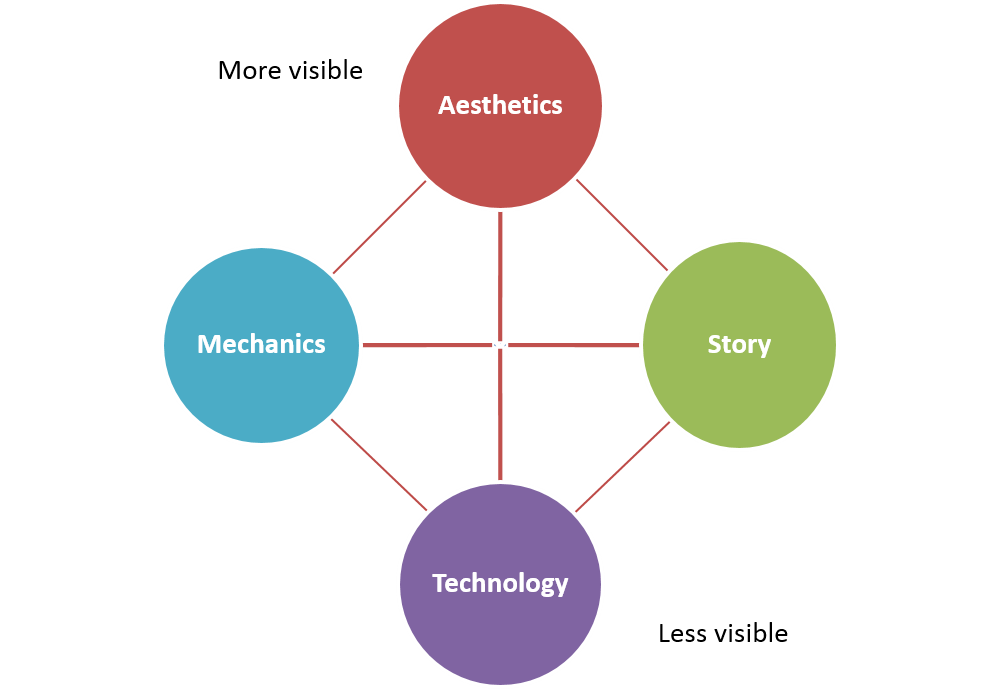
\includegraphics[width=0.85\textwidth]{images/chap-general-background/schell-game-elements.png}
 \fdireta{Schell2008}
\end{figure}

There are many ways to classify the elements that are part of a game. According to \citeonline{Schell2008}, these elements as shown in \autoref{fig:schell-game-elements} are classified in the following four basic elements:

\begin{description}
\item[Mechanics:] These are rules and procedures that are used to describe the goals of games, how game players can try to achieve them, and what happen when they try.
\item[Story:] This is the sequence of events (script) that unfold in your game. It may be pre-scripted, linear, or complex with branching and emergent. In general, the mechanics that will be used must strengthen the story, and the mechanics will also help reinforce the ideas of story.
\item[Aesthetics:] There are how your game looks, sounds, smells, tastes, and \emph{feels}. They are an important aspect of game design that have most direct relationship to a player's experience during the game (gameplay experience).
\item[Technology:] This is the materials and interactions that make your game possible. It is the medium in which the aesthetics happen, in which the mechanics will occur, and through which the story will be told. 
\end{description}

Although the elements listed above define the components of a game, the essence of a game is rooted in the interactive nature in which the users act as players \cite{Schell2008}.
The player puts his mind inside the game world, but the game world really only exists in the mind of the player.
This magical situation is made possible by the game interface, which is where player and game come together.
Thus, the goal of a good game interface is not to look nice or to be fluid, although those are nice qualities, the goal of a game interface is to make players feel in control of their experience because the purpose of a game is by itself to create an experience in the user mind.

According to \citeonline{WerbachHunter2012}, the game elements are described as smaller pieces used to build blocks that, in an integrate form, constitutes gameplay experience. Thus, these game elements are separate in three categories: dynamics, mechanics and components, described in \autoref{fig:game-elements-pyramid}.

\begin{figure}[htb]
 \caption{Hierarchical classification of game elements}
 \label{fig:game-elements-pyramid}
 \centering
 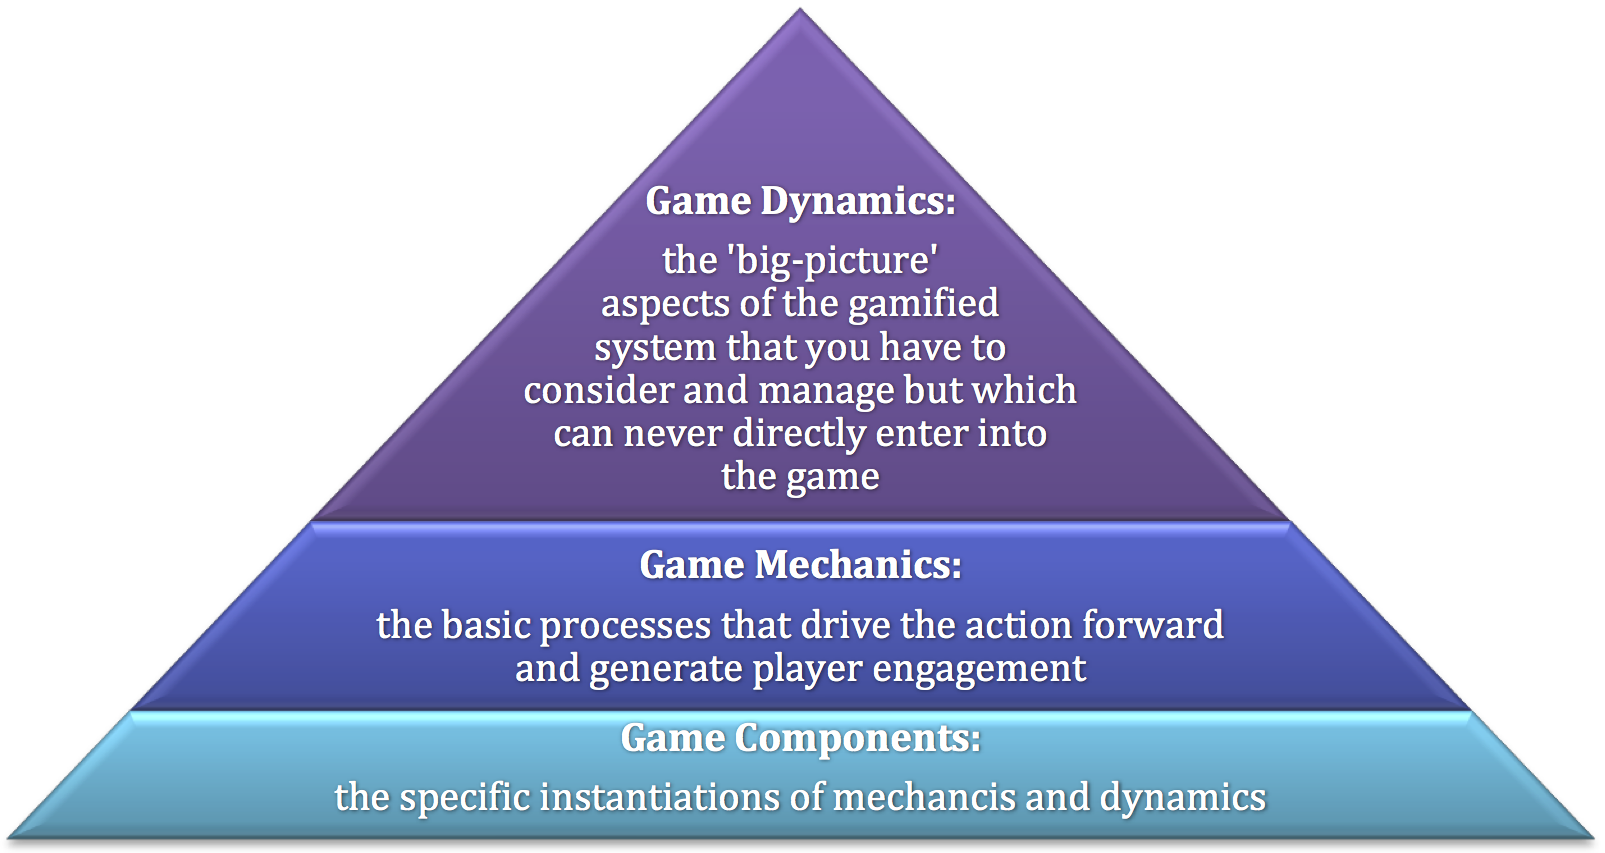
\includegraphics[width=0.85\textwidth]{images/chap-general-background/game-elements-pyramid.png}
 \fdireta{WerbachHunter2012}
\end{figure}

Based on the hierarchy of game elements showed in \autoref{fig:game-elements-pyramid}, the game elements are classified as:
\begin{description}
\item[Game Dynamics] when the game element are the big-picture aspects of the game-like system that can be to consider and manage but which you can never directly enter into the game. e.g. constraints, emotions, narrative, progression, relationships, and personalization.
\item[Game Mechanics] when the game element is part of the basic processes that drive the action forward and generate player engagement. e.g. challenges, chance, competition, cooperation, feedback, resource acquisition, rewards, transactions, turns, win-states, and profiles.
\item[Game Component] when the game element is the more-specific forms that mechanics or dynamics can take. e.g. achievements, badges, collections, leaderboards, levels, notifications, points, progress bars, quests/missions, status, teams, and virtual goods.
\end{description}

The \emph{gameplay experience}, or simply called \emph{gameplay}, is the player's interpretation of manner in which a player or players interacted in a game world \cite{SalenZimmerman2004, Lindley2004, MayraErmi2005}. Figure \ref{fig:gameplay-experience} shows the relation among the fundamental components which are part in the formation of gameplay experience. The model showed here is not intended to constitute a comprehensive analysis of all possible elements between a game and a player, the game is represented as a structure (of mechanics, story, and space) that engenders the gameplay experience in the mind of the player through a game interface. Thus, the gameplay experience happens by linking perception, cognition, and emotions when a person does actions that are motivated by the game (motivation).

\begin{figure}[htb]
 \caption{Fundamental components in the gameplay experience}
 \label{fig:gameplay-experience}
 \centering
 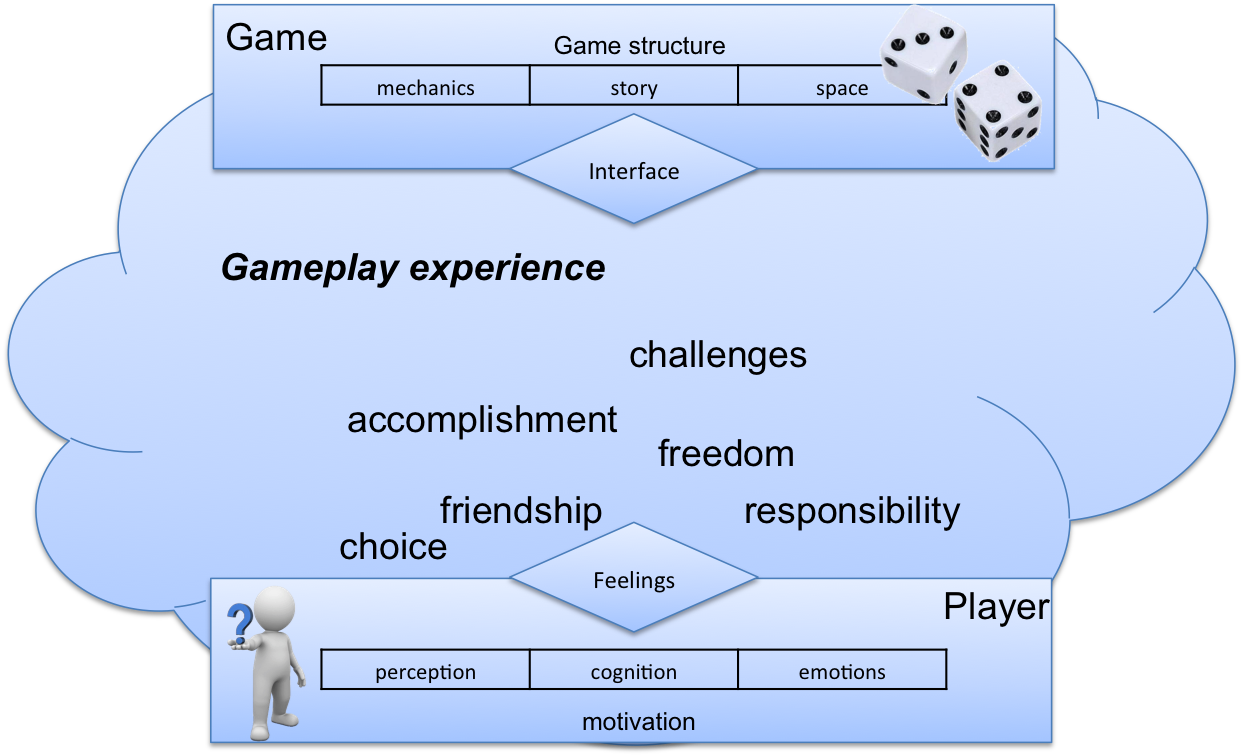
\includegraphics[width=1\textwidth]{images/chap-general-background/gameplay-experience.png}
 \fadaptada{MayraErmi2005}
\end{figure}

There are certain feelings, feelings of choice, feelings of freedom, feelings of responsibility, feelings of accomplishment, feelings of friendship, and many others, which only gameplay experience seems to offer \cite{Schell2008}. The gameplay experience is not identical in people, each person has completely different and unique experience playing a game, but the experience is imaginary. Thus, the game designers must have careful selection the proper game elements, such as game mechanics, game interfaces, among others, that are used to create certain kinds of experiences when a player interacts with them. This task is known as \emph{game design}, and it is basic when some situation, scenario or application is being gamified.

\subsection{What Is Gamification? and What Is It Not?}

While no standard conceptualization of gamification exists, most studies agree that gamification generally refers to the use of game-based elements, such as game mechanics, aesthetics, and game thinking in non-game contexts aimed at engaging people, motivating action, enhancing learning, and solving problems \cite{BorgesDurelliReisIsotani2014,  Kapp2012}. However, it is important a deeper and scientific conceptualization to identify theoretical foundations, purposes, and knowledge about how to apply gamification in practice. In this sense, based on the work of academics and industry practitioners, \citeonline{DeterdingDixonKhaledNacke2011} establish the conceptualization of gamification as the use of game design elements in non-game contexts, and \citeonline{Werbach2014} defines gamification as the process of making activities more game-like.
In other words, it covers coordinated practices that objectively manifest the intent to produce more of the kinds of experiences that typify games.
%Gamification is a process in the world manifesting that intent to create player's subjective gameplay experience as an aspect of the gamification, but not as a necessary condition.

\begin{figure}[htb]
 \caption{Situating gamification in the scope of game design technology}
 \label{fig:game-design-technology}
 \centering
 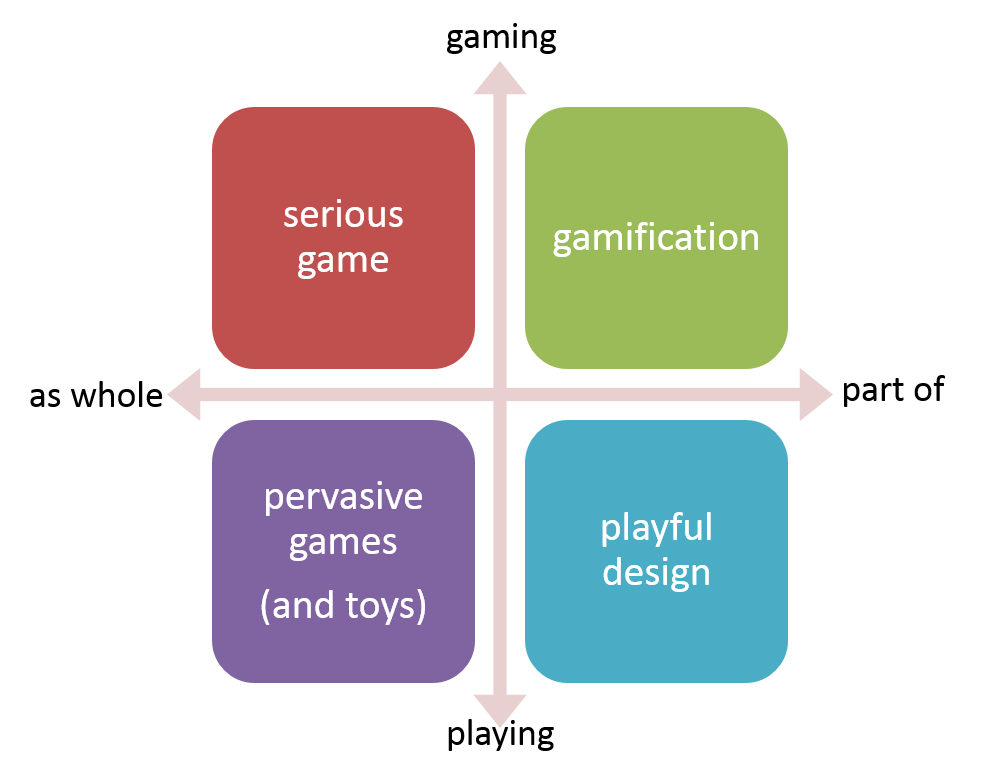
\includegraphics[width=0.85\textwidth]{images/chap-general-background/game-design-technology.png}
 \fadaptada{DeterdingDixonKhaledNacke2011}
\end{figure}


\autoref{fig:game-design-technology} shows where gamification and others game design technology are situated based on the degree of design (as whole or parts) and purpose (for playing or gaming). As we can see in the figure, gamification and serious game are similar in terms of purpose, but they differ in the degree of design, both are made for non-entertainment purposes, serious game describes the design of application as a whole game, while gamification describes the design of application as part of whole. Gamification and playful design have the same degree of design, both implements parts of application as game, while the purpose of playful design is entertainment as a desirable user experience or mode of interaction, and gamification is made for non-entertainment.

According to \citeonline{DeterdingDixonKhaledNacke2011}, gamification is related to gaming, not playing or playfulness, where playing denotes a free-form of expression, improvisational, even tumultuous recombination of behaviors and meanings. Gaming consists in the capture of playing that is structured by rules-base systems. Gamification does not describe the design of full-fledged games, gamified applications merely incorporate elements of games (also called game atoms \cite{BrathwaiteSchreiber2009}). However, these elements do not refer game-based technologies or other game related practices (e.g. as authoring tools, graphic engines), gamification is only reserved for the use of game design. The use of game design elements in gamification is for purposes other than the normal expected use as part of an entertainment game (for non-entertainment purpose).

%Game design elements are themselves difficult to specify. There is only one effort done by \citet{deterding2011from} that order from concrete to abstract levels the game design elements. Table \ref{tab:game-design-elements} summarizes the levels of abstraction identified in this study.

%\begin{table}[thbp] \footnotesize
%\begin{center}
%\begin{tabular}{|p{2.5cm}|p{7cm}|p{3cm}|} \hline
%\textbf{Level} & \textbf{Description} & \textbf{Example} \\ \hline \hline
%Game Interface Design Patterns &
%Common, successful interaction design components and design solutions for a known problem in a context including prototypical implementations. &
%Badges, leaderboards, levels \\ \hline
%Game Design Patterns and Mechanics & 
%Commonly reoccurring parts of the design of a game that concern gameplay. &
%Time constraints, limited resources, turns \\ \hline
%Game Design Principles and Heuristics &
%Evaluative guidelines to approach a design problem or analyze a given design solution. &
%Enduring play, clear goals, variety of game styles \\ \hline
%Game Models &
%Conceptual models of the components of games or game experience. &
%MDA model, game design atoms, CEGE model, challenge-fantasy-curiosity  \\ \hline
%Game Design Methods &
%Game design-specific practices and processes &
%Playtesting, playcentrinc design, value conscious \\ \hline
%\end{tabular}
%\end{center}
%\caption[Taxonomy of game design elements by level of abstraction]{Taxonomy of game design elements by level of abstraction (Adapted from \citep{deterding2011from}).}
%\label{tab:game-design-elements}
%\end{table}

\subsection{Outcomes of Gamification}
\label{subsec:outcomes-gamification}

When gamification is properly applied, a wide range of desired outcomes can be achieved, such as enjoyment, engagement, fun, satisfaction, motivation, loyalty, participation, efficiency, and behavior change \cite{HamariKoivistoSarsa2014}. In this sense, the outcomes of gamification as shown in \autoref{fig:outcomes-gamification} can be seen as: (1) the psychological outcomes (i.e. motivation, engagement, enjoyment, and fun) that are results of implemented motivational affordance (i.e. badges, points, leaderboards, and feedbacks); and (2) the behavioral outcomes (i.e. response pattern, duration of interactions, participation, and learning) that are result of psychological outcomes.

\begin{figure}[htb]
 \caption{Expected outcomes of gamification}
 \label{fig:outcomes-gamification}
 \centering
 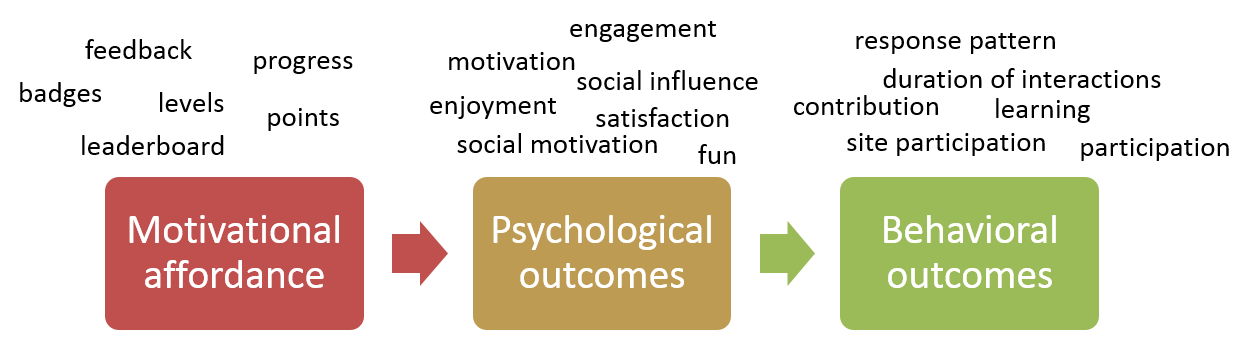
\includegraphics[width=0.85\textwidth]{images/chap-general-background/outcomes-gamification.png}
 \fadaptada{HamariKoivistoSarsa2014}
\end{figure}


In educational contexts, most studies, as shown in \autoref{qua:outcomes-gamification-education}, propose the engagement of learners as psychological outcomes, and the improving of learning as behavioral outcomes \cite{BorgesDurelliReisIsotani2014}.
For example, \citeonline{LiGrossmanFitzmaurice2012} investigated how story/theme, clear goals, feedbacks, challenge and rewards (motivational affordance) could be used to increase the engagement and enjoyment (psychological outcomes) of students, and the results showed an increase in the speed of completion of tasks (behavioral outcomes).


\begin{quadro}[htb]
\caption{Outcomes of gamification in educational contexts}
\label{qua:outcomes-gamification-education}
\centering
\footnotesize
\begin{tabular}{|p{3cm}|p{3.5cm}|p{3.5cm}|p{3.5cm}|} \hline
\textbf{Source} & \textbf{Motivational Affordances} & \textbf{Psychological Outcomes} & \textbf{Behavioral Outcomes} \\ \hline \hline
\cite{CheongCheongFilippou2013} & points, feedback, leaderboards, time constraints (challenge) & enjoyment, engagement & impact on learning (usefulness) \\ \hline
\cite{Denny2013} & badges & enjoyment, attitude towards badges & level and quality of participation \\ \hline
\cite{DominguezSaenz-de-Navarretede-MarcosFernandez-SanzPagesMartinez-Herraiz2013} & leaderboards, badges & attitude towards gamification & learning outcomes \\ \hline
\cite{DongDontchevaJosephKarahaliosNewmanAckerman2012} & clear goals, challenge, feedback, levels, story/theme & engagement, fun & effectiveness of learning \\ \hline
\cite{Fitz-WalterTjondronegoroWyeth2011} & achievements, clear goals & perceived added value of gamification, fun & exploration of the campus while interacting with the application \\ \hline
\cite{HakulinenAuvinenKorhonen2013} & badges & & impact on time management, carefulness and achieving learning goals \\ \hline
\cite{HalanRossenCendanLok2010} & leaderboards, narrative (story/theme), deadline (challenge) & difference in users' approach to virtual patient interaction & Number and duration of interactions with virtual patients, likelihood of voluntary participation to a virtual patient interaction \\ \hline
\cite{LiGrossmanFitzmaurice2012} & story/theme, clear goals, feedback, challenge, rewards & engagement, enjoyment & task performance \\ \hline
\cite{SmithBaker2011} & story/theme, rewards & & increasing knowledge about the library, its services and resources, teaching library skills \\ \hline
\end{tabular}
 \fadaptada{HamariKoivistoSarsa2014}
\end{quadro}

\subsection{Theories and Models of Motivation}
\label{subsec:theories-motivation}

As defined by \citeonline{MitchellDaniels2003}, motivation is a process what is referred as hypothetical construct associated with three general psychological processes: arousal, direction, and intensity.
The arousal is the first component caused by the need or desire to some object or state that is at least partially unfulfilled or below expectation.
This discrepancy initiates the action to satisfy the need, to obtain the desired object or to achieve the unfulfilled state. Moreover, this discrepancy is personal, and differs in each individual, different people have different needs and different things that they think are important. Thus, the second is a directional component defined by personal goals and goal discrepancies that are seen as major goads to attention and action. The third component is the intensity dimension defined by the goal difficulty and importance of arousal because some needs are more
important than others, and some goals are more difficult to attain
than others.

Having knowledge about how to motivate people, it is possible to build and formalize the proper understanding of what pushes people to interact in a gamified application, what make it fun, and why it is enjoyable. In this direction, there are different theories and models of motivation related to gamification, that are briefly summarized as follows. 

\subsubsection{Need-based Theories}
\label{subsubsec:need-theories}

There are many theories that revolve around the fulfillment of humans' needs, defined as the arousal component of motivation. 
These theories describe what make certain outcomes appear attractive, and they constitute the basic foundations of motivation. 
With relation to gamification, there are three main need theories that are detailed in the paragraphs below.

\textbf{Maslow's hierarchy of needs theory} states that a person has a pyramid hierarchy of needs that a person must satisfy from bottom to top \cite{Maslow1954,Goble1970}. As shown in \autoref{fig:maslow-pyramid}, the Maslow's need pyramid classifies the needs from basic to complex in five categories: physiological, safety, love/belonging, esteem, and self-actualization.

\begin{figure}[htb]
 \caption{Maslow's pyramid of need}
 \label{fig:maslow-pyramid}
 \centering
 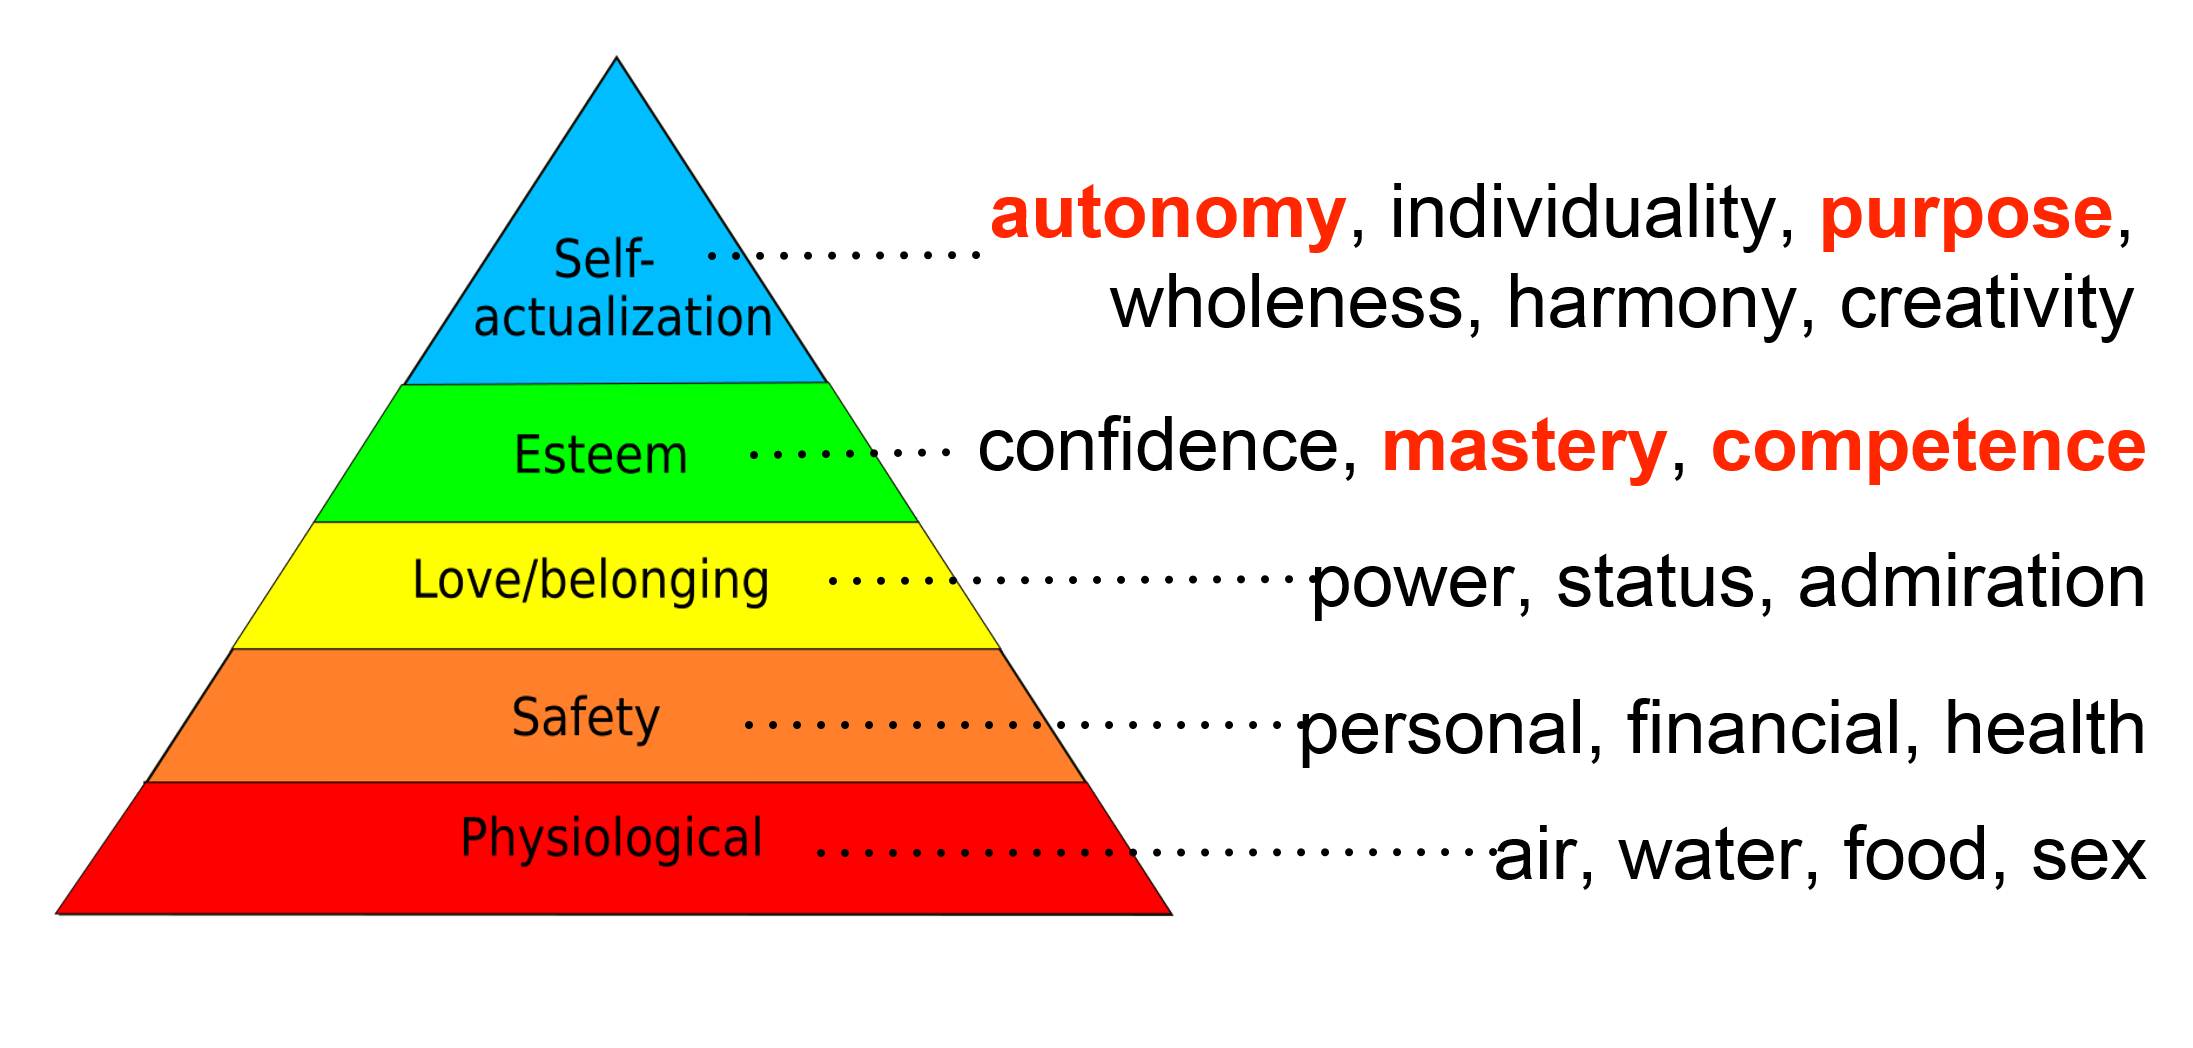
\includegraphics[width=0.85\textwidth]{images/chap-general-background/maslow-pyramid.png}
 \fadaptada{Maslow1954}
\end{figure}

According to \citeonline{Huitt2004}, only unsatisfied human needs influence behavior, if there is a deficit in a lower level, all behaviors of an individual will be oriented to satisfy this deficit. In the Maslow's need pyramid, needs are arranged in order of importance to human life, as said before from the basic to the complex. 

\textbf{Alderfer's ERG Theory}, as shown \autoref{fig:erg-theory}, condenses Maslow’s pyramid hierarchy of needs in three categories: Existence (material and physiological), Relatedness (social and external esteem) and Growth (internal esteem and self-actualization) \cite{Alderfer1969,Alderfer1972}.

\begin{figure}[htb]
 \caption{Relation between Maslow's hierarchy of needs theory and Aldefer's ERG theory}
 \label{fig:erg-theory}
 \centering
 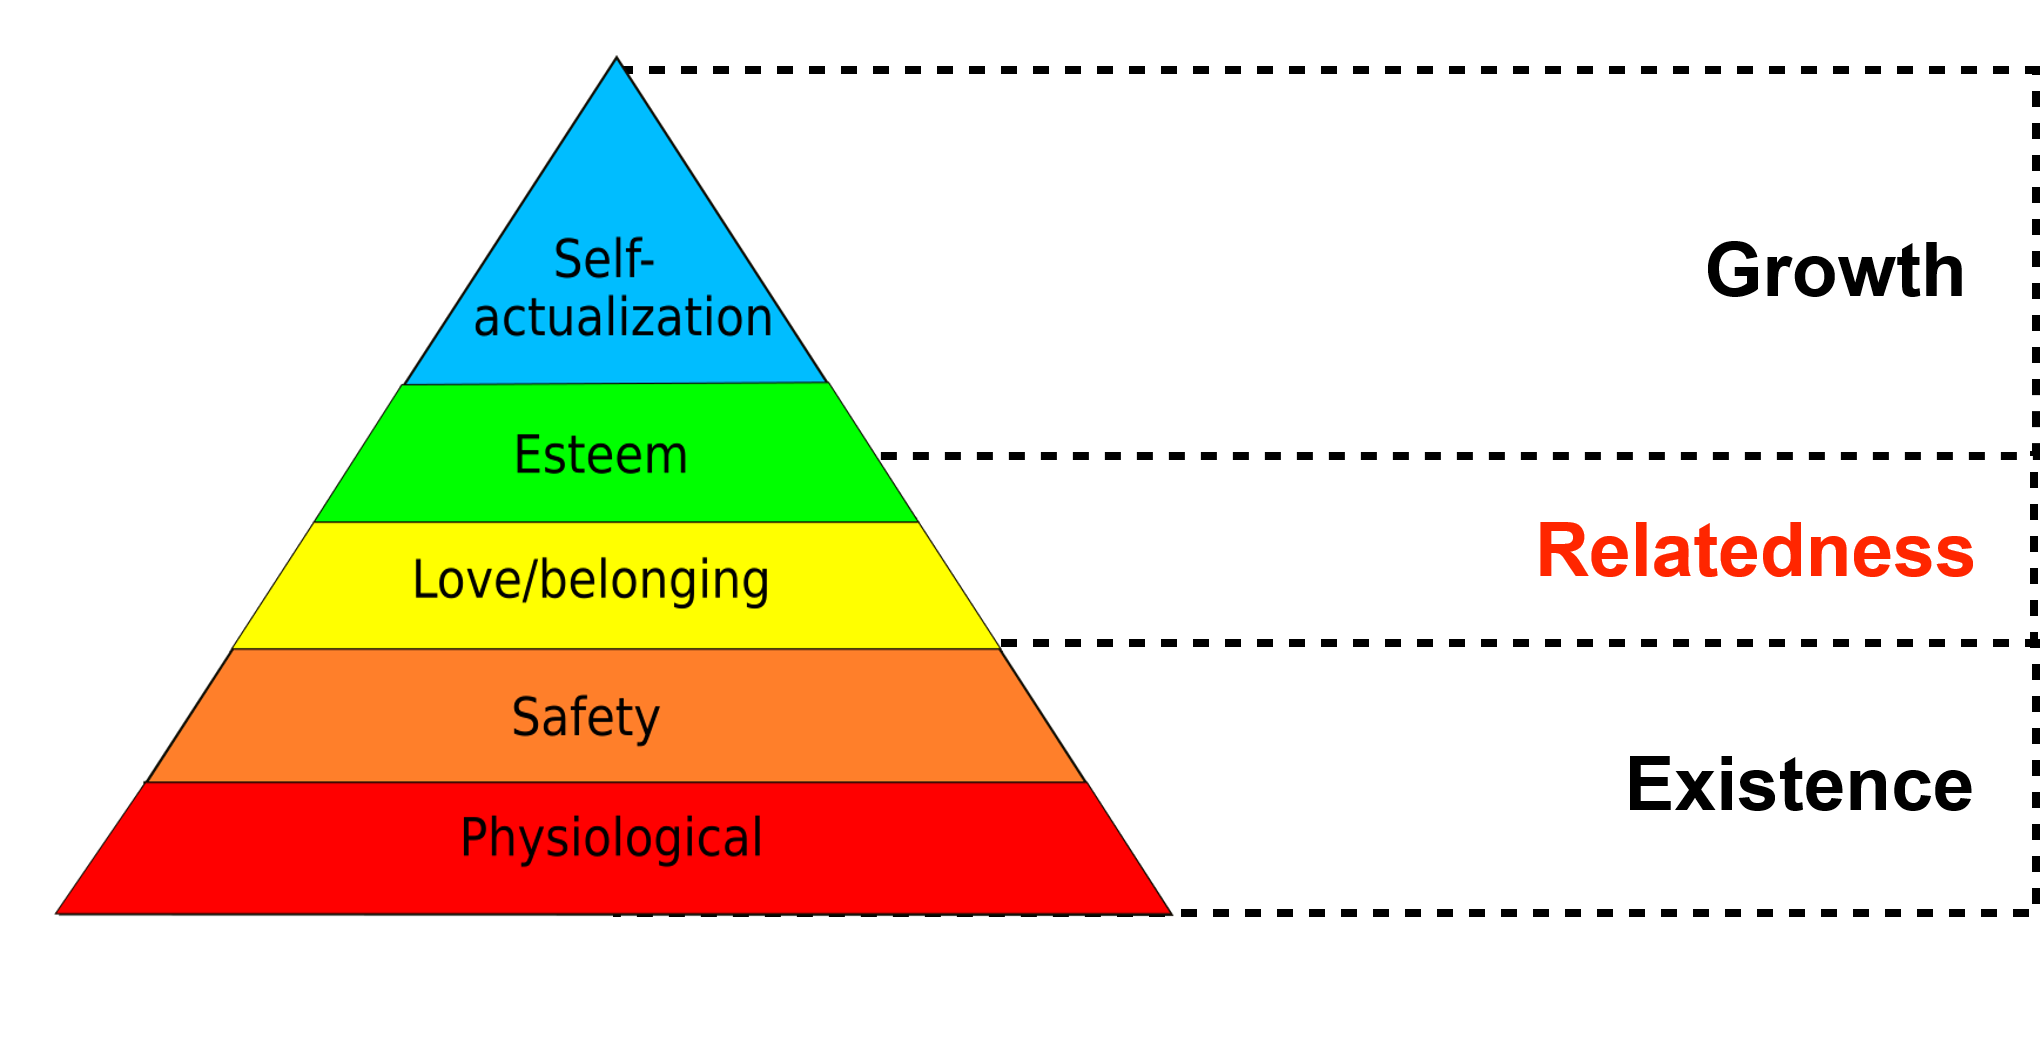
\includegraphics[width=0.85\textwidth]{images/chap-general-background/erg-theory.png}
 \fautor
\end{figure}


Different to Maslow's hierarchy of needs theory, a person can regress to a basic level from a complex level if a relatively more significant need (of complex level) is not satisfied \cite{Alderfer1972}. Thus, a person may satisfy a need at hand, whether or not a previous need has been satisfied. Finally, the theory states that the order of needs to differ for different people.

\textbf{Self-Determination Theory} (SDT) is one of the most well-known theory related to motivation. Through the understanding of needs and motivation, this theory explains the human beings' innate psychological needs for personal development and well-being, and the impact of the environment on individual's motivation \cite{DeciRyan2010,RyanDeci2000}. SDT defines three innate needs (competence, relatedness, and autonomy) that cause individual motivation, and when these needs are fulfilled they invoke great personal growth \cite{ArazyGellatly2012}.

According to SDT theory, the three needs are not learned, and they are seen as universal necessities in humanity across time, gender and culture. They are summarized as follows:
\begin{itemize}
\item \emph{Autonomy} is the need to have independence and to be able make own choices \cite{DeciRyan2010}. \citeonline{DeciVansteenkiste2004} states that autonomy does not mean to be independent of other persons. In a game, an example is to give a player freedom to make his own choices among various paths to choose.
\item \emph{Relatedness} is the need to be connected with others, iterate with them, and experience caring for them \cite{BaumeisterLeary1995}. In a game, there are many elements that allow a player socializer with other players.
\item \emph{Competence} is the need to control the outcomes and experience a sense of ability (mastery) \cite{White1959}. In a game, when a player sees a leaderboard or progress state, he or she increases their proficiency and skills.
\end{itemize}

In the SDT, there are two categories of motivation: intrinsic motivation, and extrinsic motivation \cite{DeciVansteenkiste2004}. Extrinsic motivation occurs when an external stimulus evokes a target behavior. Some of these stimulus can be rewards, threats, punishment, pressure, external regulations, and rules. The intrinsic motivation comes from individuals, and pushes them to act for the sake of the activity itself \cite{DeciRyan2010}. The intrinsic motivation occurs when the behavior is itself rewarding or engaging for the individual. The intrinsic motivators act on the human predisposition to strive for novelty and challenges, to extend and exercise one's capacities, to explore and to learn \cite{RyanDeci2000}. These intrinsic motivators include altruism, competition, cooperation, sense of belonging, love or aggression \cite{Muntean2011}.

On the one hand, the use of extrinsic motivators is a highly reliable technique for behavioral change, but the behavior disappears instantly when these external motivators are halted \cite{HaggerChatzisarantis2007}. On the other hand, intrinsic motivation is intense, and lasting engagement in the behavior, but it cannot be predicted every each person as it is internalized \cite{DeciRyan2010}. Internalization of motivation refers to the active attempt to transform an extrinsic motive into personally endorsed values. It means the assimilation of behavioral regulations that were originally external.

\subsubsection{Skinner's reinforcement theory}
\label{subsubsec:operant-conditioning}

The reinforcement theory or operant conditioning theory proposed by \citeonline{Skinner1976} states that reinforced behaviors will tend to be repeated, while punished behavior tend to be decrease and will eventually end. Thus, the operant conditioning is a process that attempts to modify behavior by positive and negative reinforcement. Therefore, through operant condition, an individual makes an association between consequences and behaviors. For example, telling a child to go to his room is a punishment frequently used to avoid the cursing.

\begin{quadro}[htb]
\caption{Forms of operand conditioning to human behavior}
\label{qua:operant-conditioning}
\centering
\scriptsize
\begin{tabular}{|c|c|c|} \hline
 & \textbf{Positive} & \textbf{Negative} \\ \hline
\multirow{4}{*}{\textbf{Reinforcement}} & \multirow{4}{*}{add appetitive stimulus} & \emph{Escape} \\
 & & remove noxious stimuli \\ \cline{3-3}
 & & \emph{Active Avoidance} \\
 & & avoid noxious stimulus \\ \hline
\textbf{Punishment} & add noxious stimuli & remove appetitive stimulus \\ \hline
\end{tabular}
 \fautor
\end{quadro}

In this sense, the reinforcement and punishment as shown in  \autoref{qua:operant-conditioning} are operant conditioning that come in two forms: positive and negative. As we can see in this table, the negative reinforcement has two forms, one related to remove the noxious stimuli (escape) and other related to avoid the stimuli (active avoidance).

%\subsubsection{Mood, Emotion and Affect Theories}
%\label{subsubsec:mood-emotion-affect-theories}
\subsubsection{Csikszentmihalyi's Flow Theory}
\label{subsubsec:flow-theory}

Csikszentmihalyi's flow theory constitutes an important theory regarding the study of affective states during active activities for intrinsic purposes, such as discussions, exercises, and learning activities \cite{SnyderLopezPedrotti2010, Csikszentmihalyi2014}. Passive activities like listening music or watching TV usually do not need individuals to actively do something. The flow theory describes the experiences of intrinsically motivated persons in tasks chose for its own sake. Thus, this theory states that in order for a task to be fully engaging it must reach an optimal mind state named flow, which is a state of optimal intrinsic motivation, full concentration, absorption and intense immersion \cite{Wu2011, Xu2011}. In other words, if a user is in flow state during the performance of a task, he or she feels naturally in control and neither overwhelmed by difficulty nor uninterested. The users in flow state experience a loss of self-awareness, forgetting about time, worry, ego and physical symptoms.

\begin{figure}[htb]
 \caption{Graph of the three-flow channel model}
 \label{fig:flow-channel}
 \centering
 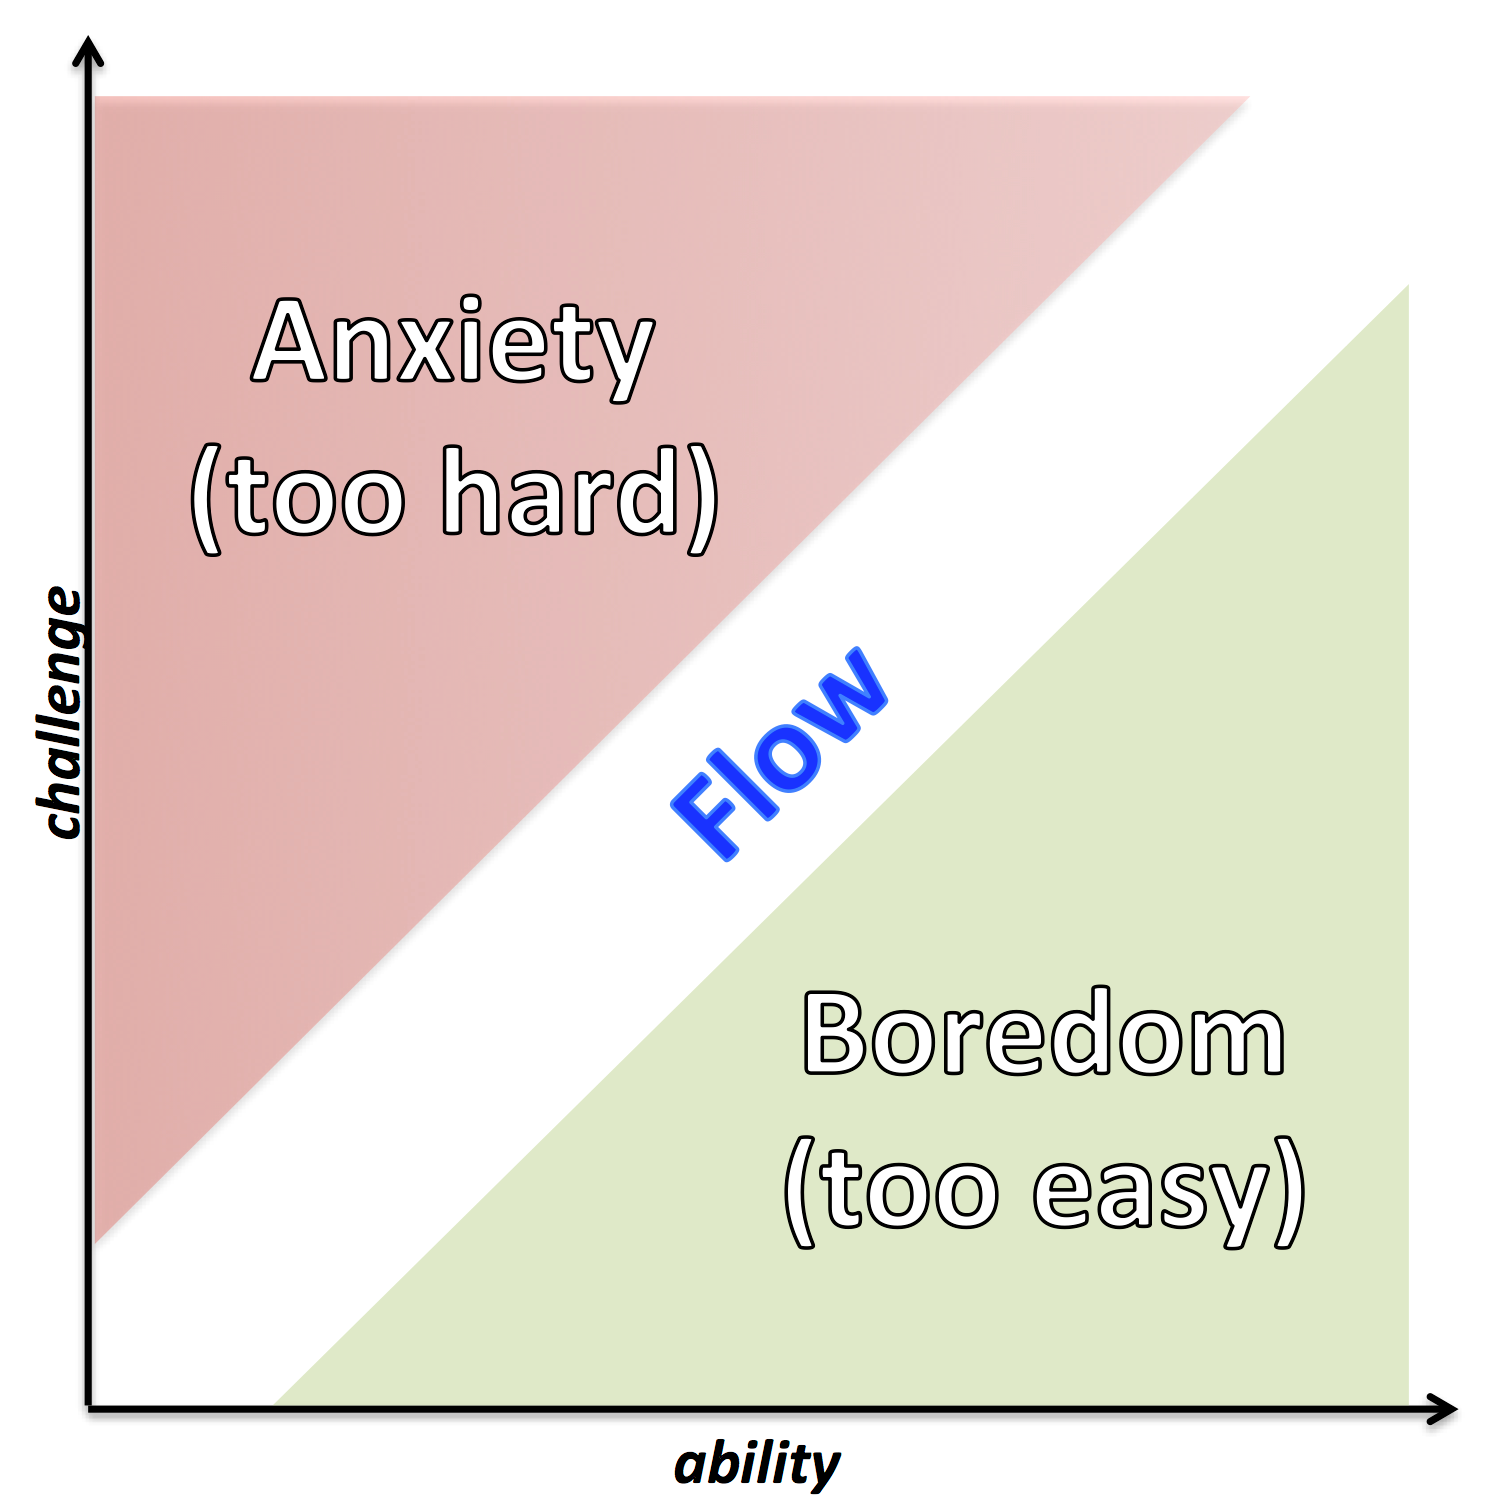
\includegraphics[width=0.55\textwidth]{images/chap-general-background/flow-channel.png}
 \fadaptada{Csikszentmihalyi2008}
\end{figure}

It is not a simple task to reach a flow state, and according to the flow theory, the following conditions must be satisfied to achieve the flow state:

\begin{itemize}
\item Clear goals, in which the expectations and rules are clearly discernable.
\item Direct and immediate feedback, in which the successes and failures of task are apparent, so that behavior can be adjusted as needed.
\item Good balance between ability level and challenge.
\end{itemize}

In the flow theory, the most important condition is accomplishing and maintaining the right balance between difficulty and ability to do some task. There must be enough challenge so that the user will not become bored but not so much that the user will feel frustrated by the complexity \cite{Csikszentmihalyi2008}. This delicate equilibrium is denominated as flow channel and is depicted on \autoref{fig:flow-channel}.

The ability to create the flow state in games and game-like systems as gamification is essential to engagement users in these applications \cite{Xu2011}. However, it is typically challenging to create activities that induce the right balance between ability and difficulty that matches all users of an application.

\subsection{Persuasion and Persuasive Design Models}
\label{subsec:persuasive-theories-persuasive-design-models}

Persuasion as a practice is as old as human existence, and it is defined as the process of influencing changes of peoples' beliefs, attitudes, intentions, and motivations toward target behaviors \cite{SeiterGass2004}. Human-to-human persuasion was broadly researched since early 400 BC when Aristotle defined rhetoric as \aspas{… \emph{the faculty of observing in any given case the available means of persuasion}} \cite{Natanson1955}. Thus, there are many persuasive models that are concentrated on addressing aim to change the mental state of the persuades through communication \cite{GueriniStockZancanaro2007}.
In the last decade, many researches pointed out that similar to a human persuader, computing technologies can be used to produce changes in human behaviors, beliefs, attitudes, intentions, and motivation in various ways of designing technology to influence these changes in different contexts, such as sports \cite{HarjumaaSegerstaahlOinas-Kukkonen2009}, health \cite{OrjiVassilevaMandryk2014}, and education \cite{LuceroZuloagaMotaMunoz2006, GohSeetChen2011}.

In this section, an overview of most relevant persuasive design models to develop computer as persuasive technologies, defined as Captology \cite{Fogg2002}, is summarized below.

\subsubsection{Fogg's Behavior Model}
\label{subsubsec:fogg-behavior-model}

According to \citeonline{Fogg2009}, for a behavior to occur, the motivation, ability, and trigger must converge at the same moment reaching the activation threshold. \autoref{fig:foggs-behavior-model} depicts the Fogg's behavior model, in which the components of model (motivation, ability, and trigger) show that, to pass the activation threshold and trigger the behavior, an event or task must be motivating and not too difficult. In this sense, the three components of Fogg's behavior model are defined as follows:

\begin{itemize}
\item \emph{Motivation} is the process used to allocate energy in actions to maximize the satisfaction of needs \cite{PritchardAshwood2008}. In this process, energy is the time and effort available to meet those needs, and needs are the magnet that drives motivation. Thus, motivation can be measured by the degree in which someone is willing or engaged in performing the behavior \cite{Xu2011}.
\item \emph{Ability} is the degree to which someone has the skills or tools to carry out the behavior \cite{Xu2011}. There are six factors that work together in the context of a trigger to define the ability, these factors are: time, money, physical effort, brain cycles, social deviance, and non-routine.
\item \emph{Trigger} is what prompts people to take a behavior. The trigger is also known with different names such as cue, prompt, call to action, request, and so on. The trigger is related to the degree to which someone is provoked to perform the behavior \cite{Xu2011}. Sometimes a trigger can from our daily routine (e.g. walking through the kitchen may trigger us to open the fridge), other times the triggers can be external, such as alarms, messages, and so on.
\end{itemize}

\begin{figure}[htb]
 \caption{Visual depiction of Foog's Behavior Model}
 \label{fig:foggs-behavior-model}
 \centering
 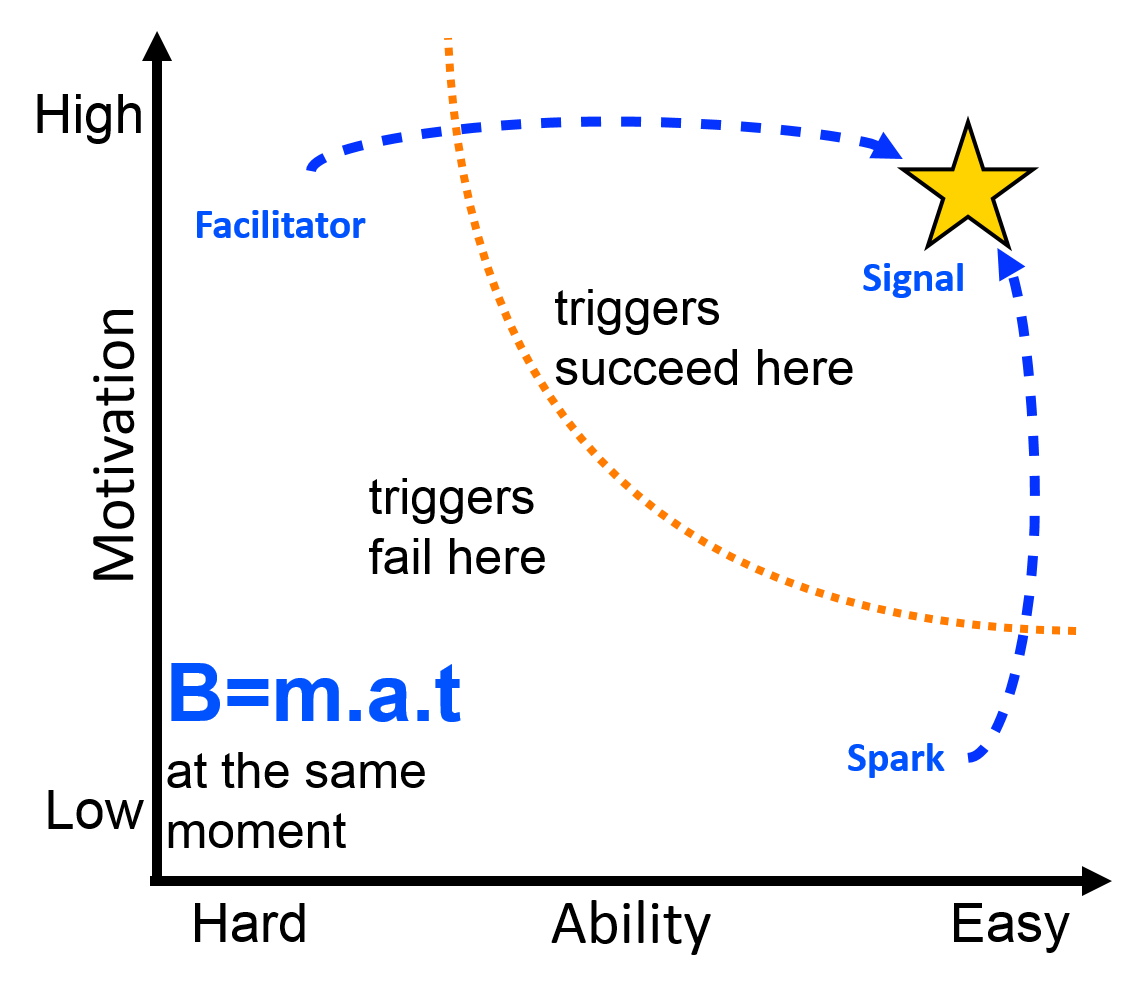
\includegraphics[width=0.6\textwidth]{images/chap-general-background/foggs-behavior-model.png}
 \fadaptada{Fogg2009}
\end{figure}

When a target behavior does not occur, at least one of those three factors is missing, or one is not enough sufficient to attain the activation threshold.
The fact, if the individual has a high motivation to accomplish the task, but if he/she does not have the ability to perform it, the behavior will not occur.
On other hand, if the individual lacks motivation to perform a target behavior, this behavior does not occur.
Having the ability and motivation alone are not enough to cause a behavior, people need triggers that them \aspas{\emph{to complete the action in a certain moment}} \cite{Fogg2009}. This trigger is not simply something that prompts or tells something to the users, independent of level of motivation and ability, a trigger at the proper time leads to the target behavior in a predictable way using this trigger as facilitator, spark, or signal.

\begin{itemize}
\item \emph{Facilitators} is a proper type of trigger for users that have high motivation but lack ability to perform certain behavior. The goal is these triggers is to make the behavior easier to do, and these facilitators can be embodied in text, video, graphics, and others medias used in games.
\item \emph{Sparks} are one type of trigger used when a person lacks motivation to perform a target behavior. Thus, triggers of this type should be designed in tandem with a motivational element. Some examples of sparks can be text or videos that inspire to hope or highlights fear.
\item \emph{Signals} is a trigger type that works best when people have both the ability and the motivation to perform the target behavior. The signals do not seek to simplify the task or to motivate people, they are only reminder because the individuals have both motivation and ability.
\end{itemize}

The game elements, more specifically game mechanics in the game design and gamification, acts as influencers that push users over the activation threshold and trigger them to perform a targeted behavior \cite{Wu2011}. In essence, a successful gamified system must cause all three elements of the behavior model to occur all at once.

\subsubsection{Persuasive System Design Model}
\label{subsubsec:psd-model}

Following the research work of Captology \cite{Fogg2002}, several models have been proposed to guide the design and evaluation of persuasive technology. The most popular of these models is the Persuasive System Design (PSD) model proposed by \citeonline{Oinas-KukkonenHarjumaa2009}. \autoref{fig:persuasive-system-design} shows the phases for the context analysis of PSD in which, from the first step of understanding the key issues behind persuasive system, the second step of analyzing the persuasion context identifies: the intent (of the persuader), the event (that triggers the persuasion) and the strategy (by which the subject is persuaded).

\begin{figure}[htb]
 \caption{Phases for the context analysis of Persuasive Systems Development}
 \label{fig:persuasive-system-design}
 \centering
 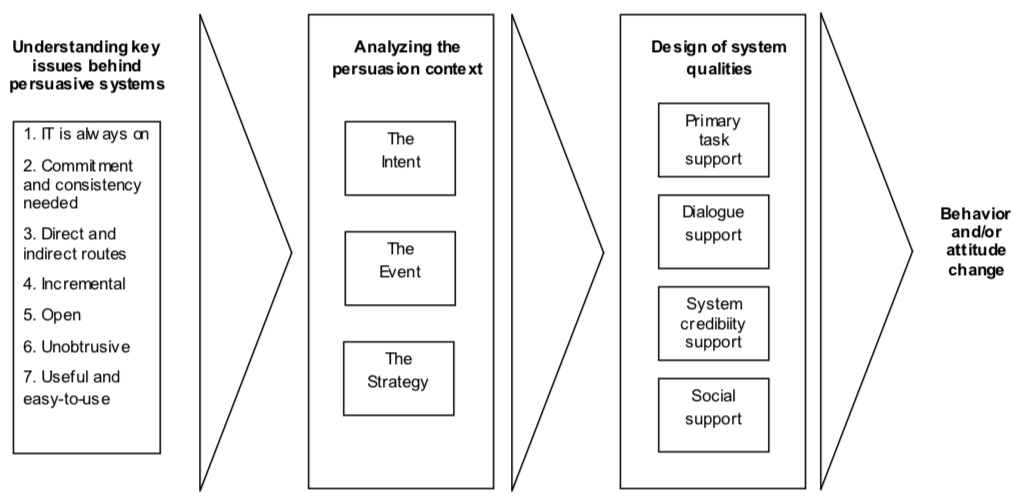
\includegraphics[width=0.85\textwidth]{images/chap-general-background/persuasive-system-design.png}
 \fdireta{Oinas-KukkonenHarjumaa2009}
\end{figure}

The third step is the design of system qualities based on design principles classified in 4 categories: primary task, dialogue, credibility, and social support.

\textbf{Primary Task Support}: techniques that help the users to achieve their goals by the principles of:

\begin{itemize}
\item \emph{Reduction}: to make the complex behavior into simple tasks by helping the users to perform the target behavior, and thus, to increase the benefit/cost ratio of a behavior.
Example: Listing a few options to be chosen, so that the user does not have to select one him/herself.
\item \emph{Tunneling}: to guide the users through a process or experience providing opportunities to persuade along the way.
Example: An interactive guide in which the step by step indicates how the user should perform a process.
\item \emph{Tailoring}: to adapt the information for the potential needs, interests, personality, usage context or other factors relevant to a user group.
Example: Giving different interface to a beginner, intermediate and advanced users.
\item \emph{Personalization}: to offer personalized content or services with a greater capability of persuasion.
Example: Adjusting personalized information in a search engine.

\item \emph{Simulation}: to provide simulations that can persuade the users to observe immediately the link between cause and effect.
Example: Before-and-after pictures of people that a people has lost weight.
\item \emph{Rehearsal}: to provide means with which to rehearse a behavior can enable people to change their attitudes or behavior in the real world.
Example: A fight simulator to help pilots in their practices.
\end{itemize}

\textbf{Dialogue Support}: techniques used in dialogue with the user in a similar way in which human-to-human interaction occur. Their principles are:

\begin{itemize}
\item \emph{Praise}: by offering this type of message, a system can make users more open to persuasion
Example: Compliments given by an application when the users perform target behaviors.
\item \emph{Rewards}: by given rewards to the users when they perform target behaviors.
Example: The users earn a virtual trophy when they complete a task.
\item \emph{Reminders}: by reminding the users of their target behavior, the users will more likely achieve their goals.
Example: A program that reminds the users to perform a target behavior.
\item \emph{Suggestion}: by offering fitting suggestions, an application has greater persuasive powers.
Example: An application that suggests the users change their habits
\item \emph{Similarity}: by imitating the users' behaviors,  people are more readily persuaded through systems that remind them of themselves in meaningful way.
Example: Using slang in the communication, an application is targeted at young people.
\item \emph{Self-monitoring}: to keep the track of the user progress/performance.
Example: Presenting a daily step count of fitness trainer.
\item \emph{Liking}: by being visually attractive for the users, a system is likely to be more persuasive.
Example: Pet-related symbols are adequate for a website targeted at pet owners.
\item \emph{Social-role}: by adopting a social role, a system is more likely to be used by the users.
Example: A virtual specialist in an application provides better support to communicate users and specialists.
\end{itemize}

\textbf{Credibility Support}: focuses in maintaining credibility on the importance of a system in which the principles are:

\begin{itemize}
\item \emph{Trustworthiness}: in a system is viewed as trustworthy increasing the powers of persuasion.
Example: A well-known 3rd party using to verify the strengths of products instead of just relying on advertising.
\item \emph{Expertise}: A system that is viewed as incorporating expertise will have increased powers of persuasion.
Example: Incorporating expertise opinions in a system.
\item \emph{Surface credibility}: People make initial assessments of the system credibility based on a firsthand inspection.
Example: A fast, clean and highly polished website without advertising feels more credible.
\item \emph{Real-world feel}: A system that highlights people or organization behind its content or services will have more credibility.
Example: A contact form in a system to support questions and/or feedback from its users.
\item \emph{Authority}: A system that leverages roles of authority will have enhanced powers of persuasion.
Example: Quotes given by an authority, such as the government in a web-site.
\item \emph{Third-party endorsements}: Third-party endorsements, especially from well-known and respected sources, boost perceptions on system credibility.
Example: Guarantee certificates provide certain quality.
\item \emph{Verifiability}: Credibility perceptions will be enhanced if a system makes it easy to verify the accuracy of site content via outside sources.
Example: Claims on a website are supported by links to relevant
sources.
\end{itemize}

\textbf{Social Support}: Social factors have ability to influence humans because they are social creatures. Thus, the following principles determine the system's persuasiveness.

\begin{itemize}
\item \emph{Social learning}: A person will be more motivated to perform a target behavior when he/she can be used to observe others performing the behavior.
Example: An application sharing the journal of others to motivate him/she to perform the behavior indicated in the journal.
\item \emph{Social comparison}: System users will have a greater motivation to perform the target behavior if they can compare their performance with the performance of others.
Example: Leaderboards in a learn-to-type application shows how well someone is doing compared to others.
\item \emph{Normative influence}: A system can leverage normative influence or peer pressure to increase the likelihood that a person will adopt a target behavior.
Example: A smoking cessation application shows pictures of newborn babies with serious health problems.
\item \emph{Social facilitation}: System users are more likely to perform target behavior if they discern via the system that others are performing the behavior along with them.
Example: A homework application shows how many children in the
user's class are doing homework at the same time.
\item \emph{Cooperation}: A system can motivate users to adopt a target attitude or behavior by leveraging human beings' natural drive to co-operate.
Example: A homework application giving multiple users parts of an equation.
\item \emph{Competition}: A system can motivate users to adopt a target attitude or behavior by leveraging human beings' natural drive to compete.
Example: An online competition, such as Quit and Win (stop smoking for a month and win a prize).
\item \emph{Recognition}: Public recognition for an individual or group increases the likelihood that a person/group will adopt a target behavior.
Example: Names of top contributors, and published on a website as user of the month.
\end{itemize}
 
\subsection{Game Design Models}
\label{subsec:game-design-models}

In gamification, several models concerning to the game design are used to describe the manners in how to combine and apply game elements in the non-game context. These models are based on  theories and models of motivation and human behavior, as well as persuasion and persuasive design model. In the following subsections, an overview of most relevant game design models are presented.

\subsubsection{Player Types Models}
\label{subsec:player-types}

The term game player (or player, for simplicity) is frequently used to describe individuals who play games, and there are different types of game players. There are people who take gaming seriously, playing full-fledged games a significant part of their daily lives. These players refer themselves as serious or hardcore gamers \cite{BosserNakatsu2006}. On the other hand, casual gamers are people ranging from occasional game players \cite{KuittinenKultimaNiemelaPaavilainen2007}. Based on characteristic that players exhibit within games such as competitiveness, sociability, exploratory behaviors, and individual personality traits, \cite{LawsJackson2002, NackeBatemanMandryk2014, Bartle2004, Marczewski2013} identify different player typologies. 

Three main typologies of player types deeply explored in this dissertation are summarized below.

\textbf{Bartle's player types} \cite{Bartle2004, Bartle1996} is the most popular classification of four-player types based on preferences of persons when they are playing a game.
By studying players of the Multi-User Dungeon (MUD) game, \citeonline{Bartle2004} identifies four players types (achievers, socializer, explorer, and killers) as shown in \autoref{fig:bartle-player-types}, in which there are two dimension of preferences: (1) the preference of interacting with other players (user-orientation) vs. exploring the game (system-orientation); and (2) the preference of unilateral action (action-orientation) vs. interaction in the game (interaction-orientation).
Employing these preferences, the four player types are defined as follows:

\begin{figure}[htb]
 \caption{Bartle's model of four-player types}
 \label{fig:bartle-player-types}
 \centering
 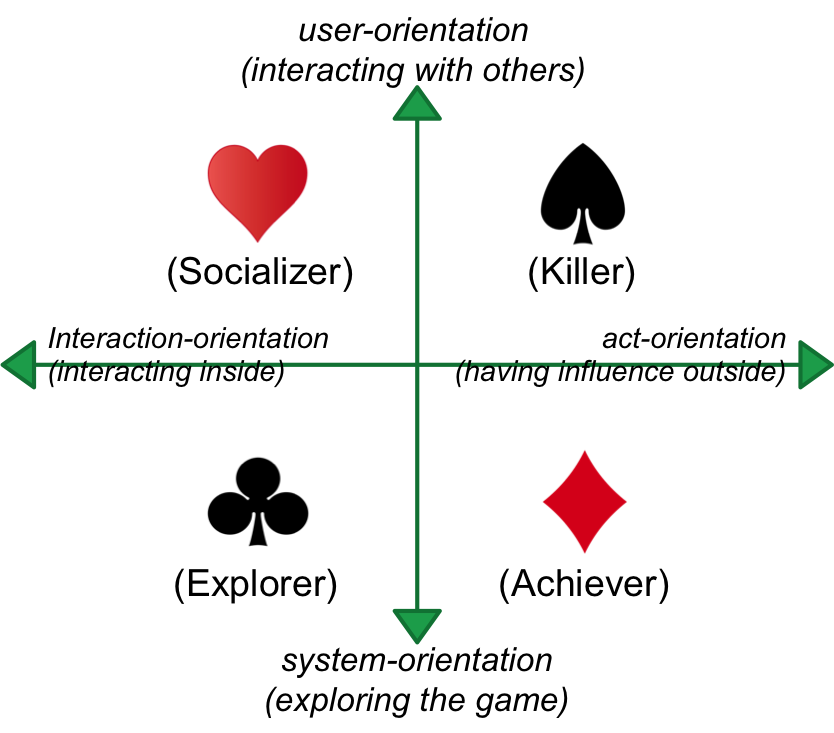
\includegraphics[width=0.55\textwidth]{images/chap-general-background/bartle-player-types.png}
 \fadaptada{Bartle2004}
\end{figure}

\begin{itemize}
\item \emph{Achievers}: These players in general play games to win, they are goal-oriented players with great sense of achievement. The gameplay experience of this player type is driven by goals that either explicitly stated by the game (for example, gathering coins, or leveling up) or personally created (for example, accumulating much money or exclusive items).

\item  \emph{Socializers}: These players are driven by communication and relationship. Socializers interacting with others players using communication tools provided by the game, and they find the greatest reward in what the others players have to say about them in the games.

\item \emph{Explorers}: These players like interact with the world, and they are driven by finding new areas and gaining new knowledge about the virtual world. The activities that a player of this type may like to include things like: exploring every corner of a map, finding interesting features such as bugs, and understanding how everything functions.

\item \emph{Killers}: These players act on other players to obtain enjoyment by attacking, killing or causing anxiety on others. Players of this player type like imposing themselves on the game to dominate others. For example, a player who likes to obtain powerful weapons to attack other players with the goal of killing the characters of other players is a killer.
\end{itemize}

\textbf{Yee's Motivational Components} \cite{Yee2006, Yee2006a} is a model of player type developed by Nick Yee who devised an experiment based on Bartle's four player types by conducting an extensive survey of Massive Multiplayer Online Role-Playing Games (MMORPGs) players for 3200 individuals who answered 39 multiple-choice questions. Based on the results of this experiments, he derived ten motivational components grouped in three main components as shown in \autoref{qua:yee-motivation-components}, where the main components are independent of each other. 

\begin{quadro}[htb]
\caption{Motivational components revealed by the factor analysis in the Yee's experiment}
\label{qua:yee-motivation-components}
\centering
\scriptsize
\begin{tabular}{|c|c|c|} \hline
\textbf{Achievement} & \textbf{Social} & \textbf{Immersion} \\
(\emph{mastery need}) & (\emph{relatedness need}) & (\emph{autonomy need}) \\ \hline \hline
\textbf{Advancement} & \textbf{Socializing} & \textbf{Discovery} \\
progress, power,  & casual chat, helping others, & exploration, lore, \\
accumulation, status & making friends & finding hidden things \\ \hline
\textbf{Mechanics} & \textbf{Relationship} & \textbf{Role-Playing} \\
numbers, optimization, & personal, self-disclosure, & story line, character history, \\
templating, analysis & find and give support & roles, fantasy \\ \hline
\textbf{Competition} & \textbf{Teamwork} & \textbf{Customization} \\
challenging others, & collaboration, groups, & appearances, accessories, \\
provocation, domination & collaboration, groups, & appearances, accessories, style, color schemes \\ \hline
& & \textbf{Escapism} \\
& & relax, escape from reality \\ 
& & avoid reality problems \\ \hline
\end{tabular}
 \fadaptada{Yee2006}
\end{quadro}

With the SDT theory as background and the mapping showed in \autoref{qua:yee-motivation-components} (autonomy need for achievement component, mastery need for immersion component, and relatedness need for social component), \citeonline{Yee2006a} points that Bartle's player types conflicted with the results analyzed through factor analysis. He states that socializing and role-playing are two independent motivations, while Bartle proposed that people who like chat and make friends are also people who like to role-play. While Bartle proposed that achievers and griefers (killers) are separate types, there is correlation between advancement and competition that defines the desire of achievers and killers, respectively. The explorer defined by Bartle as people who enjoy both exploring the world and gathering information is in reality two different kinds of people defined by the two separate factors: discovery, and mechanics. Finally, the immersion component is a motivation that did not exist in Bartle's type.

These motivations are not solely for MMORPGs but they are also applicable to other game-like systems such as gamification. Through the incorporation of these principles, a gamified system will induce larger amounts of user engagements. However, it does not define a component related with the purpose need widespread by the theory proposed by \citeonline{Pink2011}. The purpose need is a general class of need that varies from person to person, it is behind all 10 components.

\textbf{Marczewski's player types} \cite{Marczewski2015a, Marczewski2015d} expands the Bartle's model through the addition of one dimension related with type of motivation (intrinsic motivation, extrinsic motivation). As show in \autoref{fig:marczewski-player-types} (a), Marczewski describes eight player types, four of whom are intrinsic motivated (socializer, free spirits, achiever and philanthropists) and four extrinsic motivated (networker, exploiter, consumer and self seeker). According to \citeonline{Marczewski2013}, Bartle's player types is useful but flawed, at the end, a gamified system is not a MUD game where all users want to participate, and rewards plays an important role to define whom can be engaged with extrinsic motivators like badges and trophies.

\begin{figure}[htb]
 \caption{Marczewski's eight-playe and six-player types models}
 \label{fig:marczewski-player-types}
 \centering
 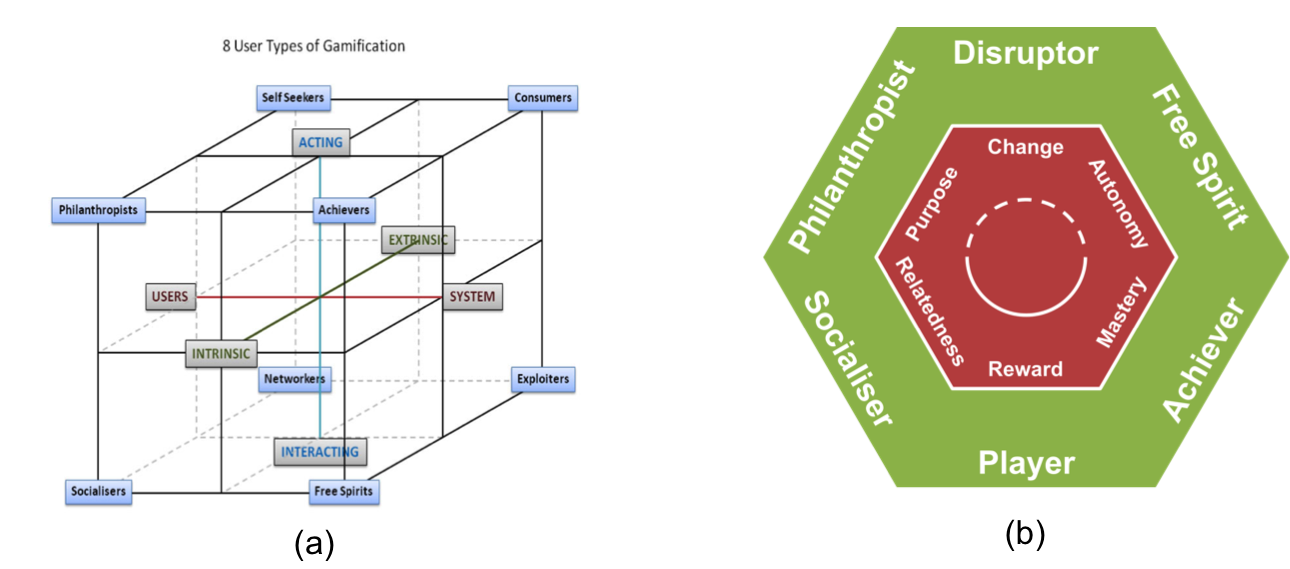
\includegraphics[width=0.9\textwidth]{images/chap-general-background/marczewski-player-types.png}
 \fadaptada{Marczewski2013}
\end{figure}

Based in the four needs defined in SDT theory \cite{DeciRyan2010} and the theory proposed by \citeonline{Pink2011} (Relatedness, Autonomy, Mastery, and Purpose), Marczewski redefines the eight-player types model to six-player types model as shown in \autoref{fig:marczewski-player-types} (b). He defines four basic intrinsic player types: Achiever, Socializer, Philanthropist, and Free Spirit that are respectively motivated by relatedness need, autonomy need, mastery need, and purpose need. Next, the player type \emph{player} groups the extrinsic player types (Self-seeker, Consumer, Networker, and Exploiter) as the players who are motivated by rewards. They will do similar thing to the intrinsic motivated player types, buy only if there is a reward at the end of it. Finally, the player type \emph{disruptor} is a group of players that act in a system motivated by change. They like to disrupt a system in some way, and rather than a single type, this player type is a group, in which there are four types: Griefer, Destroyer, Influencer, and Improver that are related with Philanthropist, Achiever, Socializer, and Free Spirit, respectively.

\subsubsection{MDA model}
\label{subsec:mda-model-need-theories}

In game design, the Mechanics-Dynamics-Aesthetics (MDA) model \cite{HunickeLeBlancZubek2004} as shown in \autoref{fig:mda-model} is a tool used to analyze game-like systems. It formalizes the consumption of games by breaking them down into mechanics, dynamics, and aesthetics, in which the \emph{mechanics} are the base components of the game, its rules, and elements  related with basic action that a player can take in the game, such as algorithms and data structures. The \emph{dynamics} are the run-time behavior of the mechanics acting on player input. The \emph{aesthetics} are the emotional responses evoked in the player, such as challenge, discover, fantasy, and fellowship.

\begin{figure}[htb]
 \caption{MDA Model: Mechanics, Dynamics and Aesthetics model}
 \label{fig:mda-model}
 \centering
 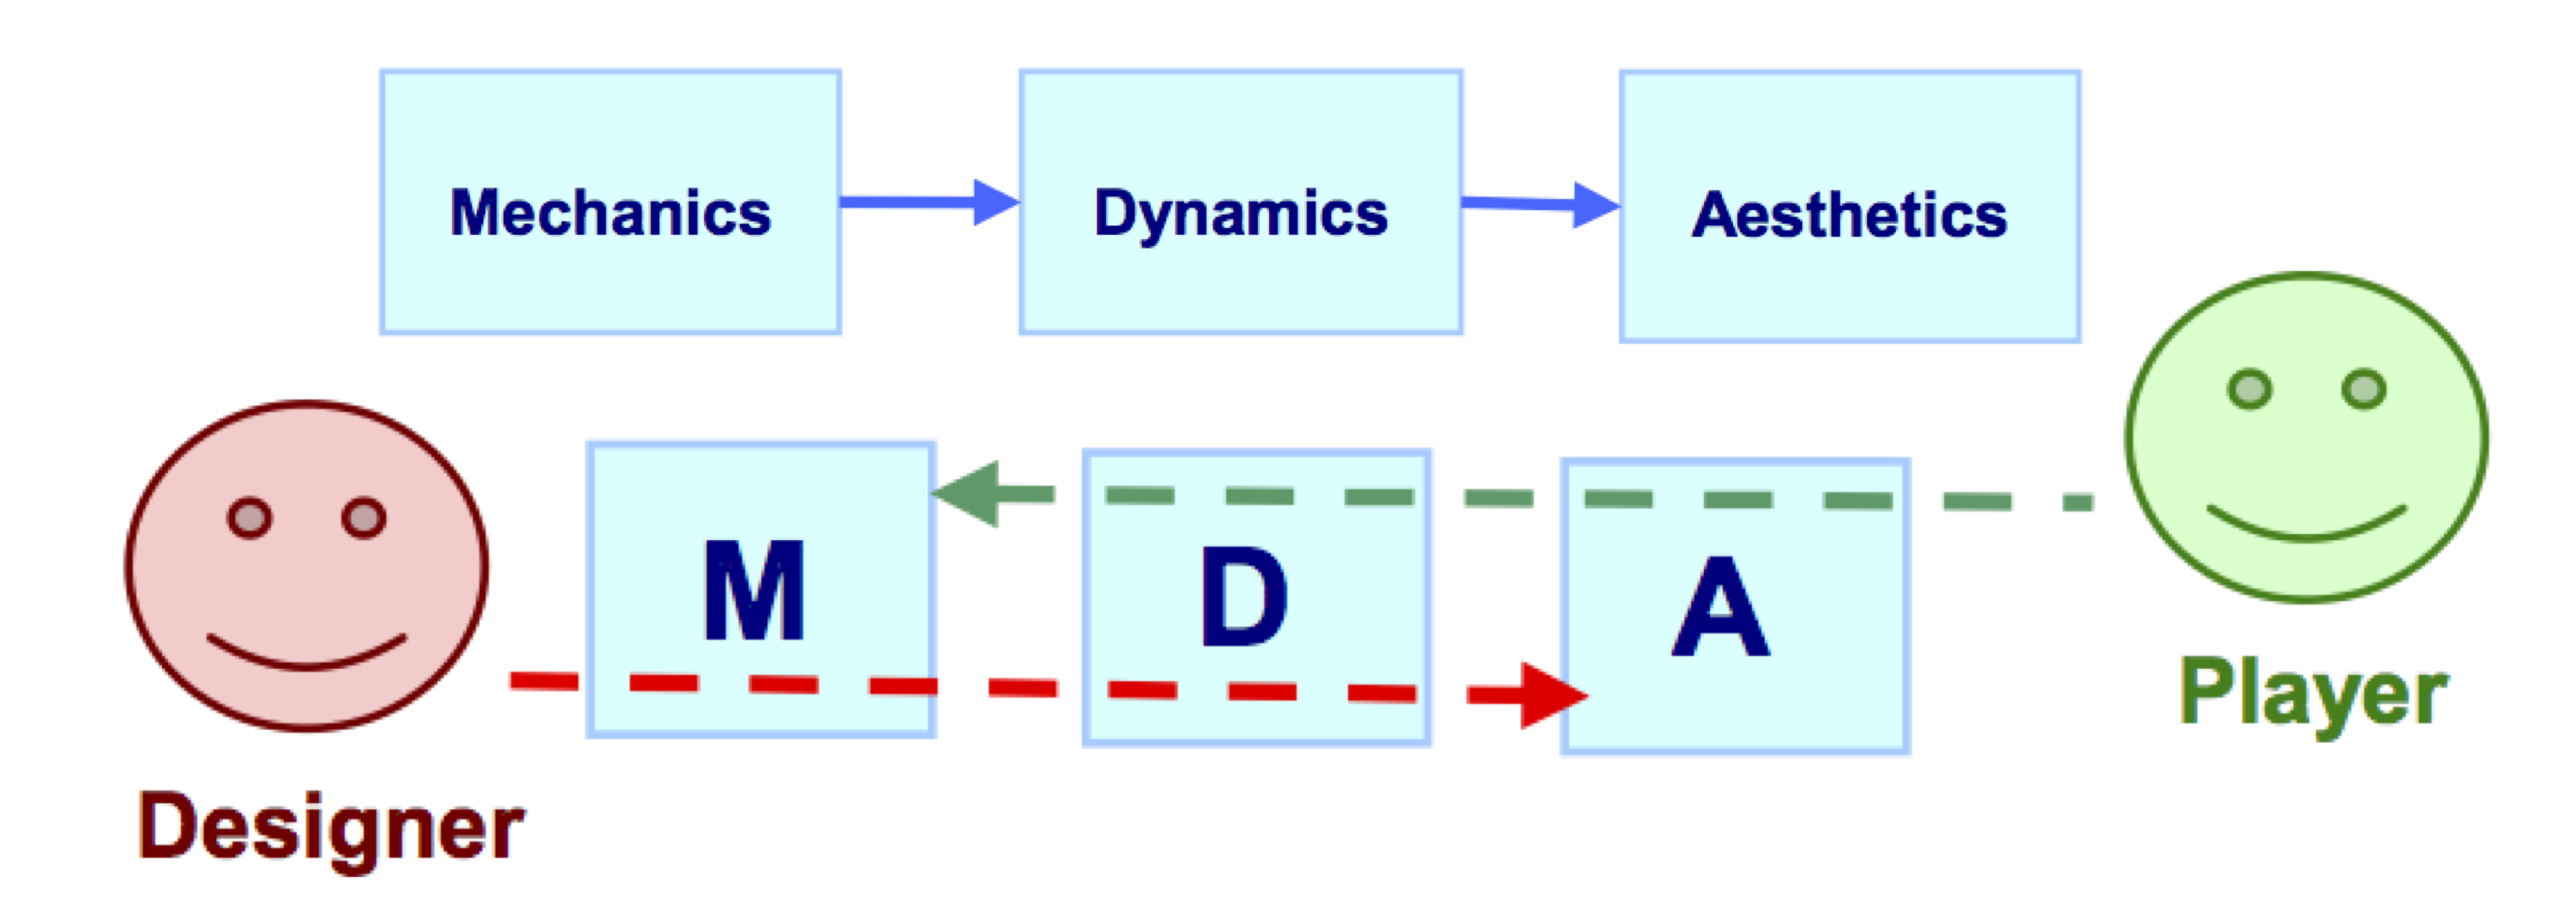
\includegraphics[width=0.85\textwidth]{images/chap-general-background/mda-model.png}
 \fdireta{HunickeLeBlancZubek2004}
\end{figure}

According to this model, the mechanics itself is not as important inside a game-like system as the dynamics and aesthetics. The authors of MDA model state that \aspas{\emph{thinking about games as designed artifacts helps frame them as systems that build behavior via interaction}.} Thus, a game-like system must provide multiple aesthetics depending on its goals. Therefore, it is important that the dynamics correspond with the aesthetics to provide an optimal environment in which the player can develop the desired behaviors, attaining the goals of game-like system. In this sense, \citeonline{Bunchball2010} propose a framework of gamification showed in \autoref{fig:bunchball-framework} that sets the relationship between game mechanics and human desires (aesthetics in MDA model).

\begin{figure}[htb]
 \caption{Human desires vs. Game mechanics}
 \label{fig:bunchball-framework}
 \centering
 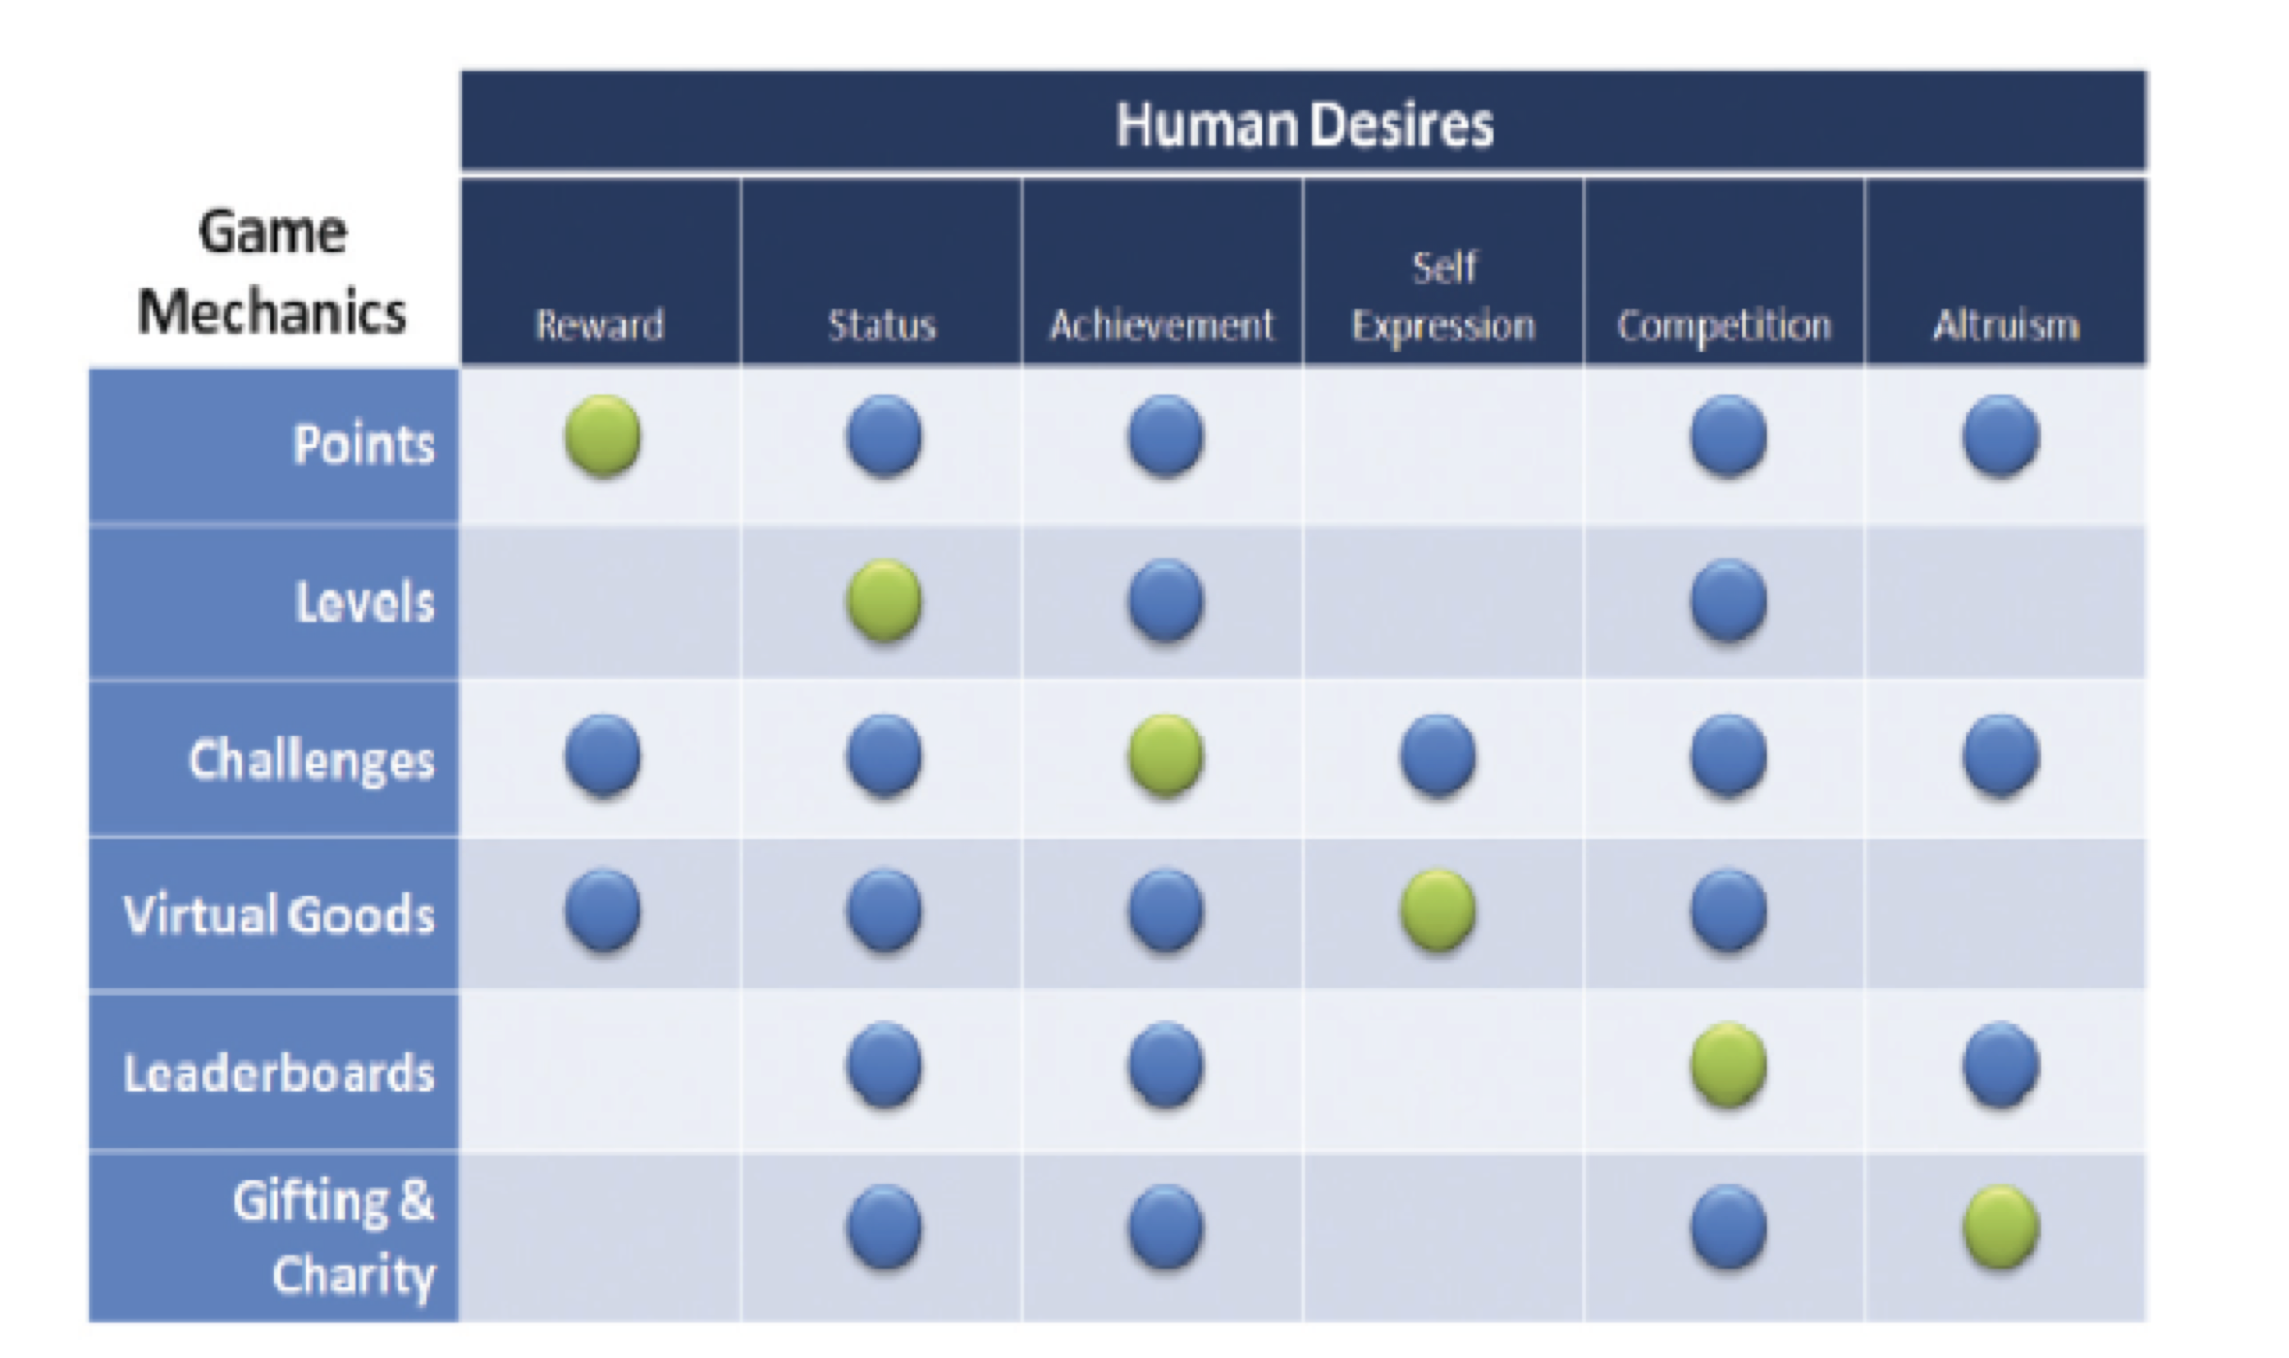
\includegraphics[width=0.85\textwidth]{images/chap-general-background/bunchball-framework.png}
 \fdireta{Bunchball2010}
\end{figure}


In the same way of the framework proposed by \citeonline{Bunchball2010}, as shown in \autoref{fig:sdt-game-elements}, we can define the relationship between some game elements and the psychological needs defined in the SDT theory. Thus, the competence need is excellently supported by game elements, such as progression tool, levels system, and point system, because they contain sophisticated mechanics that provide granular and timely feedback in term of indicators to satisfy the competence need. The relatedness need is satisfied by social interactions that have always been an important part of game-like systems through the game elements such as collaboration tool, social connection tool, social discovery, and competition tool. As the most of games placed players in the role of fictional characters providing a wide range of in-game choices through the game elements such as unlockable system, creativity tool, customization tool, and exploration tool, these elements provide support to satisfy the need of autonomy.

\begin{figure}[htb]
 \caption{Relation between game elements and SDT theory}
 \label{fig:sdt-game-elements}
 \centering
 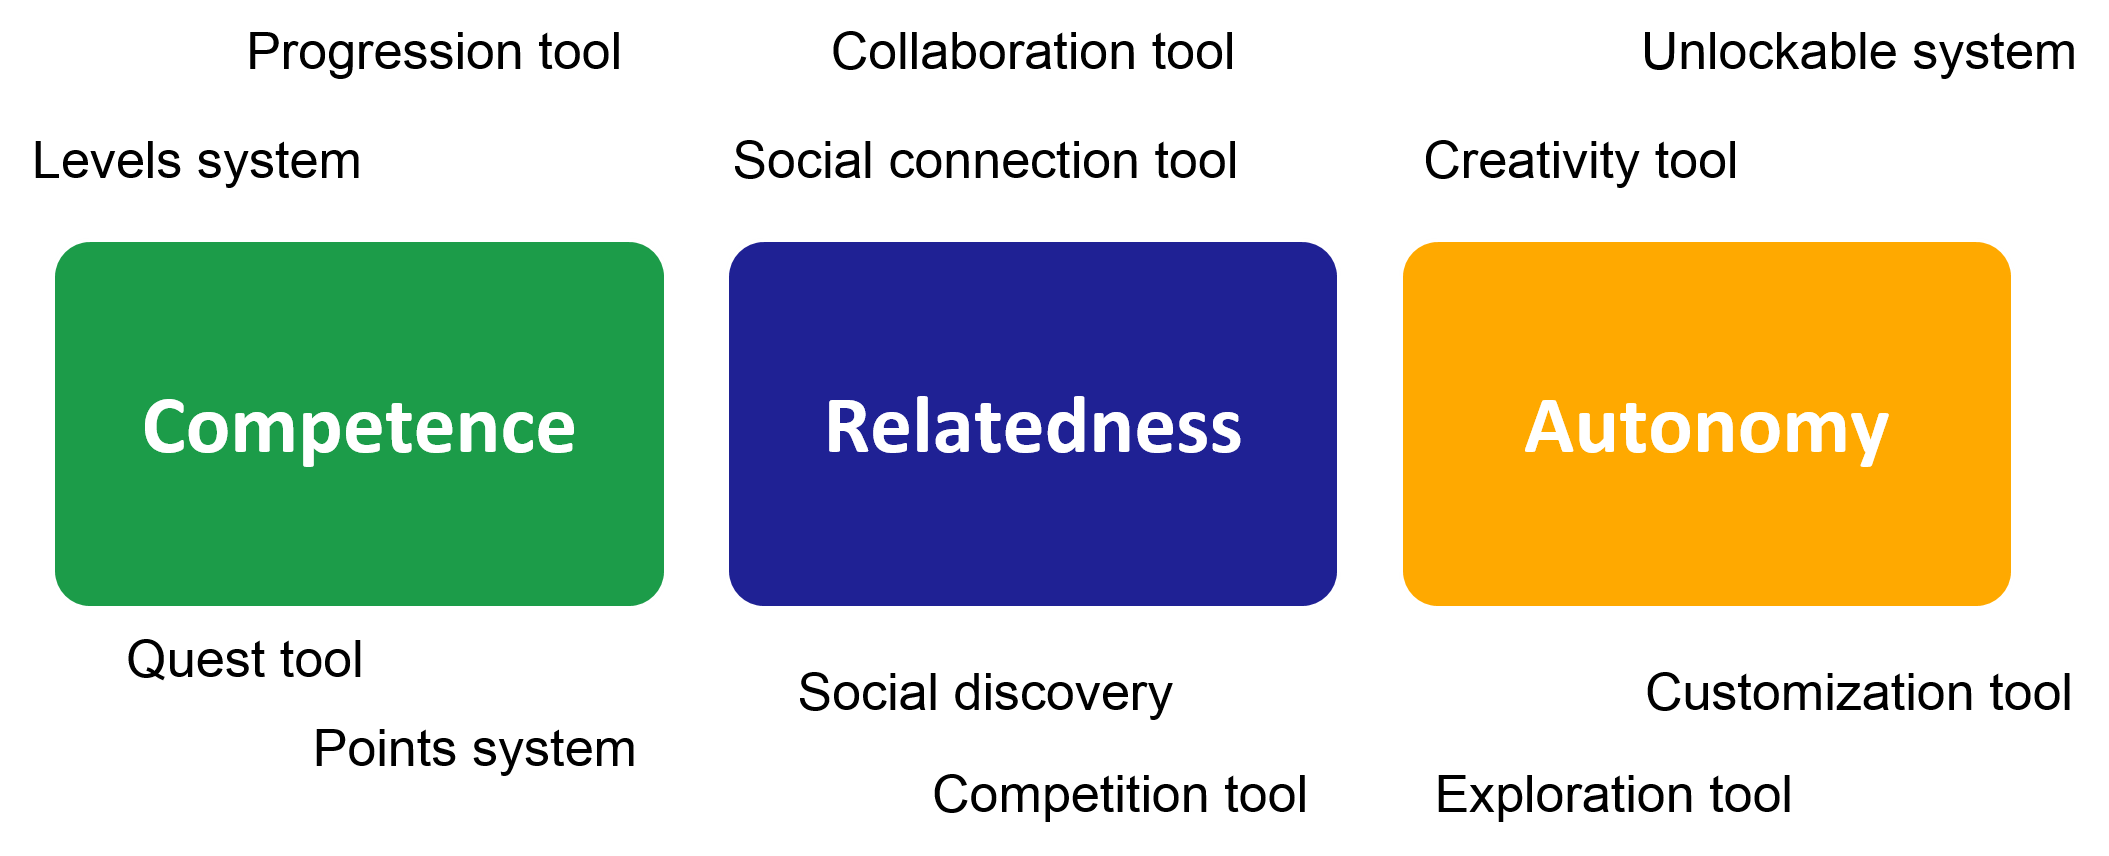
\includegraphics[width=0.85\textwidth]{images/chap-general-background/sdt-game-elements.png}
 \fautor
\end{figure}

\subsubsection{Persuasive Game Design Models}
\label{subsub:persuasive-game-design-models}

Developing persuasive technology in the form of games has become a common practice. These types of games referred as persuasive games have been designed with the the primary purpose of changing  players' behaviors, feelings, or thoughts. In the last decade, several persuasive games have been developed by researchers as a novel approach to modifying users' behaviors. For example, \aspas{\emph{What Remains}?} is a persuasive game in which using stories are used to personalize the Alzheimers' patients care giving \cite{CadamuroVisch2013}, \aspas{\emph{Smoke}?} is a persuasive game aimed to support players in smoking cessation \cite{KhaledBarrNobleFischerBiddle2007a}, and \aspas{\emph{OrderUP}!} is a persuasive
game that motivates healthy eating habits \cite{GrimesKantrooGrinter2010}.

Despite the growing interest of researchers in using and develop persuasive games, little attention has been given to develop models that would help the designers to design persuasive games and/or tailored these games to increase their efficacy at achieving their intended objective of motivating behavior change. In the following paragraphs, a model-driven persuasive game design proposed by \cite{OrjiVassilevaMandryk2014} is summarized.

\textbf{Model-driven Persuasive Game Design}: It is a model developed following the steps indicated in the model-driven approach to persuasive game design proposed by \cite{Orji2014}. This model consists in guidelines for tailoring persuasive games based on the BrainHex player-type model \cite{NackeBatemanMandryk2014}. Therefore, the best and worst persuasive strategies, as shown in \autoref{qua:mpg-best-worst-strategies}, for each one of the seven player types of BrainHex model were identified in the Model-driven persuasive game design.


\begin{quadro}[htb]
\caption{Best and worst persuasive strategies for the player types of BrainHex model}
\label{qua:mpg-best-worst-strategies}
\small
\centering

\begin{tabular}{|l|L{6.5cm}|L{6.5cm}|}
\hline
\multicolumn{1}{|c}{\textbf{Player Type}}&
\multicolumn{1}{|c|}{\textbf{Best strategy}}&
\multicolumn{1}{c|}{\textbf{Worst strategy}}\tabularnewline
\hline

Achiever&
\textbf{Cooperation}, reward, self-monitoring, and suggestion&
\tabularnewline \hline

Conqueror&
\textbf{Competition and comparison}, simulation, personalization, self-monitoring and suggestion&
\tabularnewline \hline

Daredevil&
\textbf{Simulation}&
\textbf{Self-monitoring and suggestion}, competition and comparison\tabularnewline \hline

Mastermind&
\textbf{Self-monitoring and suggestion}, competition and comparison, personalization, simulation, customization&
\tabularnewline \hline

Seeker&
\textbf{Customization}, personalization, competition and comparison, praise&
\tabularnewline \hline

Socializer&
\textbf{Cooperation}, competition and comparision&
\textbf{Self-monitoring}, praise, customization\tabularnewline \hline

Survivor&
\textbf{Self-monitoring and suggestion}, competition and comparision&
\textbf{Cooperation}, reward, customization\tabularnewline \hline


\multicolumn{3}{r}{\tiny Strategies presented in order of strength (bold are the higest)}\tabularnewline
\end{tabular}
\fadaptada{Orji2014}
\end{quadro}


After to identify the best and worst persuasive design for each player type of BrainHex model, the persuasive game design strategies have been associated to the game elements for the building of the model-driven persuasive game design as shown in \autoref{qua:mpg-strategies-game-elements}.

\begin{quadro}[htb]
\caption{Mapping of persuasive game design strategies to common game elements}
\label{qua:mpg-strategies-game-elements}
\small
\centering
\begin{tabular}{|L{4.5cm}|L{10.5cm}|}
\hline
\multicolumn{1}{|c}{\textbf{Persuasive Strategy}}&
\multicolumn{1}{|c|}{\textbf{Game Elements}}\tabularnewline
\hline

Praise&
Level, pride
\tabularnewline \hline

Cooperation&
Pride, communal discovery, social fabric of game, viral game mechanics, companion gaming
\tabularnewline \hline

Competition and comparison&
Status, envy, countdown, leaderboard
\tabularnewline \hline

Reward&
Physical goods, virtual items, rewards schedules, lottery, free lunch, points, bonuses
\tabularnewline \hline

Simulation&
Appointments, leaderboards, achievements, status, epic meaning, behavior momentum, urgent optimism, blissful productivity
\tabularnewline \hline

Personalization&
Cascading information theory, epic meaning, privacy
\tabularnewline \hline

Customization&
Shell game, discovery, epic meaning
\tabularnewline \hline

Self-monitoring and suggestion&
Quest, achievement, level, loss aversion, repeat simple action
\tabularnewline \hline

\end{tabular}
\fadaptada{Orji2014}
\end{quadro}


%\subsubsection{Feedback and Engagement Loops}
%\label{subsec:feedback-engagement-loops}

%Feedbacks include anything from indication of progress, records of accomplishments, and comments on their manner of achieving goals \citep{nahl2012technology}. In these sense, based on the operant conditioning proposed by \citet{skinner1976about}, a positive feedback loops in a game amplify something, whereas a negative feedback loops will reduce something. According to \citet{marczewski2013feedback}, feedback loops as shown in Figure \ref{fig:feedback-loops} (a) are constructed with two or more cyclical phases, in which the user firstly performs an action; next, something happens  as reaction; and finally, the user experience is modified.

%\begin{figure}[thbp]
%\begin{center}
%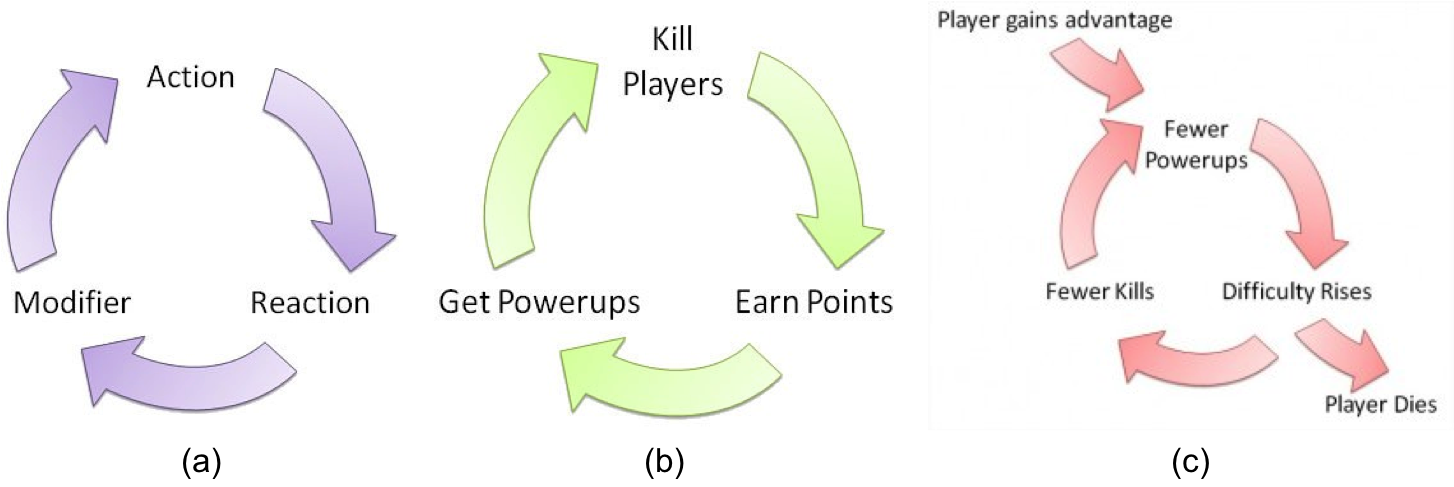
\includegraphics[width=0.95\textwidth]{feedback-loops.png}
%\caption[Basic feedback loop, example of positive feedback loop, and example of negative feedback loop]{(a) Basic feedback loop, (b) Example of positive feedback loop, and (c) Example of negative feedback loop (Adapted from \citep{marczewski2013feedback}).}
%\label{fig:feedback-loops}
%\end{center}
%\end{figure}

%In a multiplayer shooting game, an example of a positive feedback loop is showed in Figure \ref{fig:feedback-loops} (b), where an action to kill other players gives points that lead to get powerups, like increasing speed or strength. Figure \ref{fig:feedback-loops} (c) shows an example of negative feedback loop that is used when a player gains advantage over rivals. In this example, by reducing the ability to find health packs or powerful weapons, the game gives fewer powerups to the player. The difficulty rises for advance player as reaction to this action, and as consequence, there are fewer kills, leaving the less skilled player better chance of winning. This kind of balancing in games helps to keep novice players engaged.

%The engagement loops \citep{werbach2012for} as shown in Figure \ref{fig:engagement-loop} is a cycle used to define "what the players do, why they do it, and what the system does in response." Based on the Skinner's theory \citep{skinner1976about} and the Fogg's Behavior Model \citep{fogg2009a}, this cycle describes the sequence of events after each action at the micro level of a gamified system. The engagement loop starts with a player being motivated by a game element (as trigger), and as consequence, the player performs behavior, doing actions. Each one of these actions provokes a response from the system, such as rewarding point/badges or providing feedback. In general, this response is defined by a feedback loop, increasing the player's motivation which then pushes him or her to act again.

%\begin{figure}[thbp]
%\begin{center}
%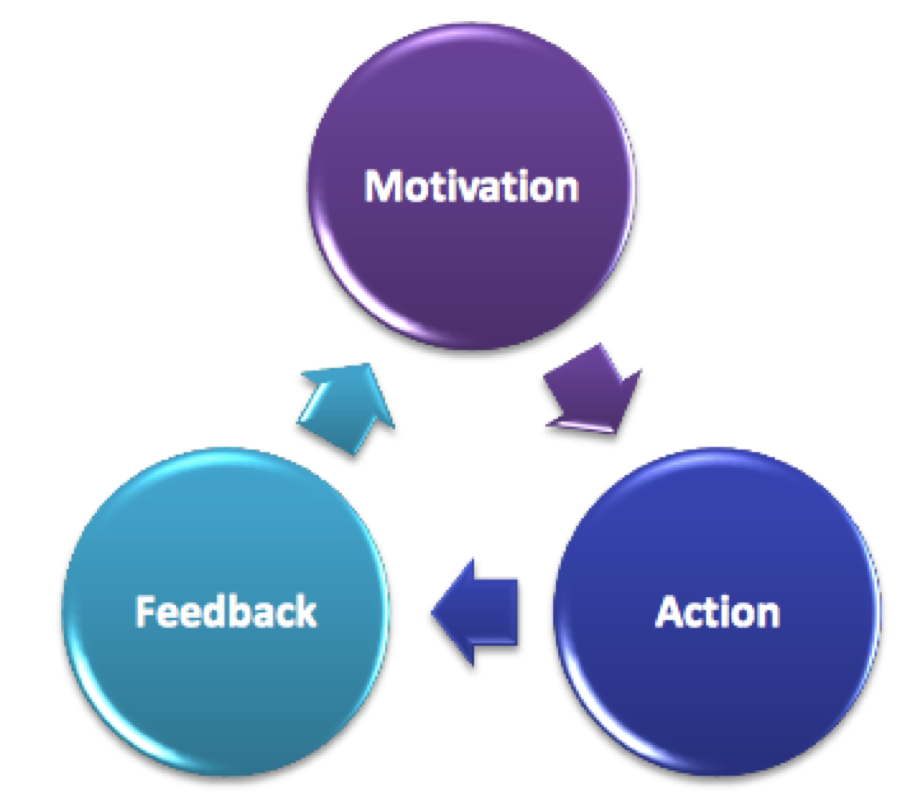
\includegraphics[width=0.55\textwidth]{engagement-loops.png}
%\caption[Engagement cycle]{Engagement cycle (Taken from \citep{werbach2012for}).}
%\label{fig:engagement-loop}
%\end{center}
%\end{figure}

%\subsubsection{Progression Steps: Player's  Journey and Flow Theory}
%\label{subsec:player-journey}

%According to \citet{kim2010designing}, good games take the player on a journey toward mastery as shown in Figure \ref{fig:player-journey}, the gameplay experience in these games changes over time in meaningful ways. Kim suggests the use of different gameplay experiences to meet player’s needs. When player is newbie, it is necessary an onboarding experience, in which the game teaches the ropes and sets expectations for what’s to come. To turn newbies into regulars, the triggers, activity loops and feedback systems build a habit-building experience. For enthusiast player, who has mastered the system and want to go deeper, it is necessary a mastery experience. 

%\begin{figure}[thbp]
%\begin{center}
%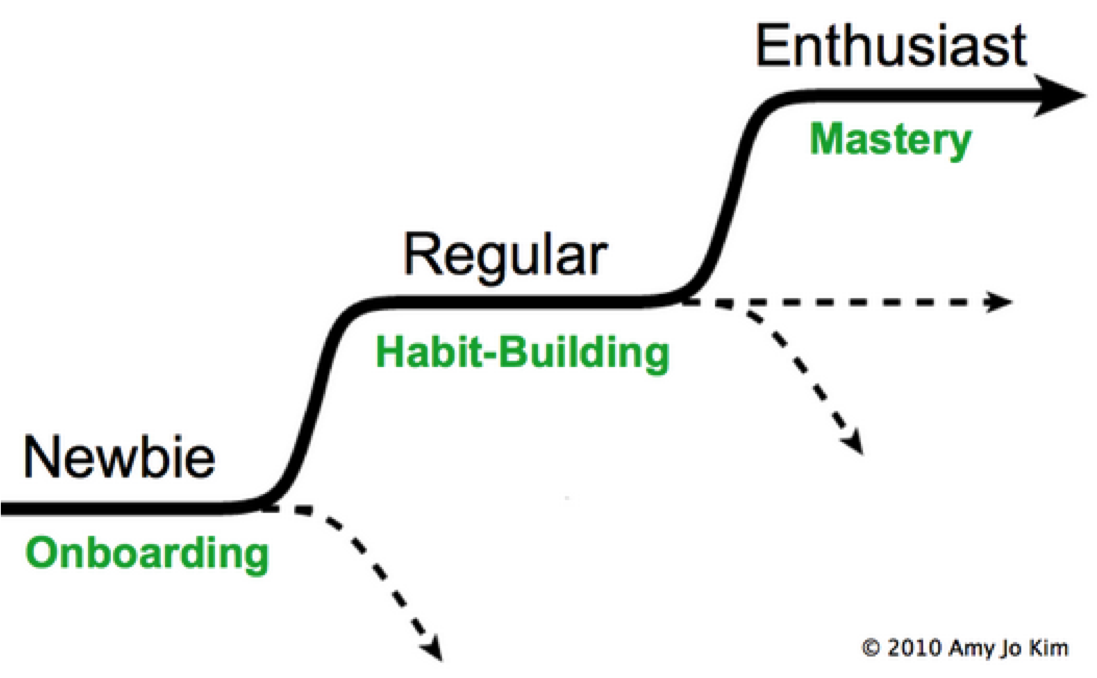
\includegraphics[width=0.55\textwidth]{player-journey.png}
%\caption[Amy Jo Kim's player journey]{Amy Jo Kim's player journey (Taken from \citep{kim2010designing}).}
%\label{fig:player-journey}
%\end{center}
%\end{figure}

%Based on the combination of flow theory and the player's journey, \citet{werbach2012for} describes the user's transition from the moment they join the system through to the end of the game. Figure \ref{fig:progression-stairs} gives an overview of how the gameplay experience is modified by a gradual escalation of difficulty. In order to retain the users at the start, the commencement of the game should be simple, informative and should guide the users to understand the basic functionality of the application. The progression cycles commence and increase the difficulty at variable rates when the users understand how to navigate the application, giving a habit-building experience. To give mastery experience in the gameplay, the \emph{rest} period or plateau is included at the commencement of each cycle to let the users to catch their breath after the sudden increase in difficulty and giving players time to put the new skills to use. At the end of each rest period, there is a final challenge, commonly known as \emph{the boss fight} that needs a larger amount of effort to complete it compared to regular missions. However, when the boss fight is completed, it is provided greater satisfaction and motivation. The boss fight completes the end of each cycle or level, and at this point the user continues to the next rank where the cycle commences again with a higher level of complexity.

%\begin{figure}[thbp]
%\begin{center}
%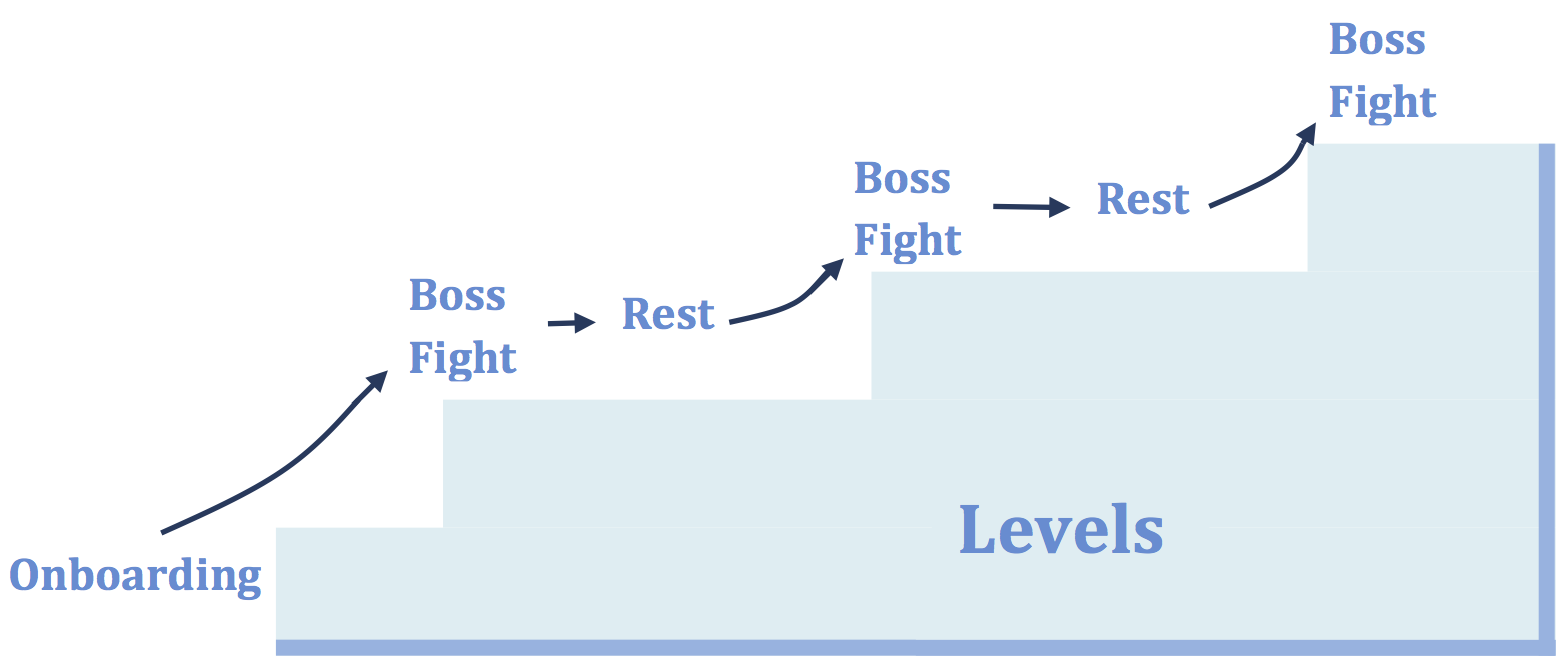
\includegraphics[width=0.85\textwidth]{progression-stairs.png}
%\caption[Progression stairs]{Progression stairs (Taken from \citep{werbach2012for}).}
%\label{fig:progression-stairs}
%\end{center}
%\end{figure}

%In the context of education, learners in the flow state frequently experience positive affect and better scores/performances compared with other learners who are in a similar situation but not in the flow state \cite{BaydasKarakusTopuYilmazOzturkGoktas2015, IbanezDiSerioVillaranDelgadoKloos2014, ShernoffCsikszentmihalyiSchneiderShernoff2014}. For example, several empirical studies conducted by D’Mello, Graesser, and colleagues using intelligent tutoring systems (e.g. AutoTutor) have shown strong positive correlations between learning gains, confusion, and flow state \cite{D'MelloGraesser2012}. Another example is the study of Choi et al., where participants used a web-based e-learning system in a program on Enterprise Resource Planning. The data of this study revealed that flow experiences were directly linked with learning outcomes and leaners’ attitude towards e-learning.

%According to previous findings, having an explicit formalization of the minimum and maximum difficulty/challenge levels to maintain the learners' flow is one of the key features needed to promote more effective and robust learning in different scenarios \cite{Esteban-MillatMartinez-LopezHuertas-GarciaMeseguerRodriguez-Ardura2014, FulmerD'MelloStrainGraesser2015 ,LinehanBellordKirmanMorfordRoche2014}. 


%To support the design of better learning scenarios that are pedagogically sound and can keep learners in a flow state, it is essential during the instructional design process to take into account the level of difficulty of learning objects and to link learning objects with theories that describe leaners’ growth. Unfortunately, this task requires specialized knowledge about instructional/learning theories, Flow Theory, and Affect Theory, and the skills to apply this knowledge in an integrated manner in order to select adequate learning objects and design effective learning scenarios that match students’ abilities. 

%To support the design of authoring tools that help instructional designers with the proper selection of levels of challenges that keep the participants in flow, in this paper we propose a framework to integrate the learner’s growth process and Flow Theory through a new theory-based model, named GMIF: Learner’s Growth Model Improved by Flow Theory. This model explains and describes the necessary conditions under which learners are able to learn more effectively based on learning theories, while keeping the ability-challenge balance of tasks defined in the Flow Theory. In particular, the GMIF has been used to create algorithms that help to automatize the selection of proper learning objects for specific learning situations.

%In a collaborative learning scenario, the challenge of designing adequate activities and selecting learning objects is even harder. If the instructional designer selects problems and learning objects that are too difficult (or too easy) for students, it will hinder students’ interactions, demotivate students, and lead students to not want to work in groups over time (Challco, Moreira, Mizoguchi, & Isotani, 2014; Isotani, Inaba, Ikeda, & Mizoguchi, 2009). For instance, consider a scenario where a student (the tutor) interacts with another student (the tutee) to solve a given problem (i.e. a selected learning object). In this situation, the tutor will learn by using his knowledge/skills to demonstrate how to solve a problem and the tutee will learn by following the tutor’s guidance. If the problem is too hard or the sequence of activities is not created to help students to collaborate, the tutor will not have the sufficient skill level or knowledge to solve and guide the tutee in the resolution of the problem. As a result, the learning scenario will cause emotional distress in both tutor and tutee, and the desired learning outcomes will not be achieved. 

%To support the design of better learning scenarios that are pedagogically sound and can keep learners in a flow state, it is essential during the instructional design process to take into account the level of difficulty of learning objects and to link learning objects with theories that describe leaners’ growth. Unfortunately, this task requires specialized knowledge about instructional/learning theories, Flow Theory, and Affect Theory, and the skills to apply this knowledge in an integrated manner in order to select adequate learning objects and design effective learning scenarios that match students’ abilities. 

%To support the design of authoring tools that help instructional designers with the proper selection of levels of difficulty that keep the learners in flow, in this paper we propose a framework to integrate the learner’s growth process and Flow Theory through a new theory-based model, named GMIF: Learner’s Growth Model Improved by Flow Theory. This model explains and describes the necessary conditions under which learners are able to learn more effectively based on learning theories, while keeping the ability-challenge balance of tasks defined in the Flow Theory. In particular, the GMIF has been used to create algorithms that help to automatize the selection of proper learning objects for specific learning situations.

%we present related works on the application of Flow Theory in educational settings. Following that, we present the GMIF, offering a detailed description of our framework that integrates the LGM and Flow Theory. 



%The related work and frameworks presented in the previous paragraph are important for guiding educators and game designers to create better learning situations. Nevertheless, they were not created to automate the process of learning design and do not have the necessary formalization to be implemented and included as a feature in a learning design authoring tool. This means that, if an instructional designer wants to maintain the learner's flow state, he/she will need to do so manually, without any computational support. Such a manual approach is infeasible to be carried out when there is a need to plan personalized sequences of activities for a class of students with different needs, using a database with multiple learning objects (e.g. games, texts, videos, images, etc.) and taking into consideration several pedagogical approaches to support flow experiences. Toward the automation of detecting and using flow state to create better learning experiences, Lee and colleagues provide adaptive learning contents by selecting appropriate problems based on the three-channel flow model \cite{LeeJhengHsiao2014}. They propose an automatic flow detector where the three-channel flow model is built based on features related to affective dimensions (i.e. valence and arousal) and interactions (i.e. mouse click duration, keystroke duration) with learning software.


%%%%%%%%%%%%%%%%%%%%%%%%%%%%%%%%%%%%%%%%%%%%%%%%%%%%%%
\section{Ontologies and Ontology Engineering}
\label{sec:ontologies-and-ontology-engineering}

%This formalization is achieved through ontology engineering in which the similarities and differences of these concepts are identified to describe their application in the gamification of CL scenarios and the building of gamification model for CL scenarios.



%In Section \ref{sec:relevant-technologies}, we presented the fundamental concepts about ontologies and ontology engineering. In this section, we detail these concepts and the techniques to create ontologies. The most of the concepts and ideas presented in this section come from the tutorial on ontology engineering published in three parts in \cite{mizoguchi2003part, mizoguchi2004tutorial, mizoguchi2004part}.

\subsection{What is an ontologies? and Why is an ontology important?}
\label{subsec:ontologies}

For philosophers, the definition of ontology came from the Greek \aspas{\emph{being, that which is},} present participle of the verb \aspas{\emph{be},} and \aspas{science, study, and theory}, is the philosophical study of the nature of being, becoming, existence, or reality, as well as the basic categories of being and their relations \cite{Wikipedia2014}. In computer science, for \citeonline{Gruber1993}, an ontology is defined as an explicit specification of a conceptualization in which the conceptualization refers to the meaningfulness of concepts and their relationship given the context of the target world. \citeonline{SwartoutTate1999} defines an ontology as the basic structure or armature around a knowledge base that can be built. As the knowledge bases are composed by facts of a given domain \cite{Hayes-RothWatermanLenat1983}, an ontology is an framework in which these facts are represented. For \cite{GuarinoOberleStaab2009}, an ontology is not a simple representation of concepts and their relations. An ontology contains restrictions defined through axioms in which these axioms are formal logical expressions that validate and check the consistency of domain. Finally, an ontology constitute agreements to achieve the mutual understanding of the target domain in a human and computer understandable manner \cite{Mizoguchi2004a}.

The definitions of ontology presented above also indicate the reasons \aspas{\emph{why}} many researches and practitioners have been attracted to develop and use ontologies as knowledge source in powerful and intelligent computational systems and applications. In these applications, an ontology first provide a common conceptual structure that enables the development of sharable and reusable knowledge-based by computer-based mechanisms and procedures, and second an ontology facilitates the interoperability of information enabling them to merge and integrate data from different sources.

\citeonline{WongLiuBennamoun2012, SugumaranStorey2002} define the fundamental components of an ontology as: individuals, classes, attributes, and relations. Individuals are instances or objects that constitute the basic or ground level of ontologies. The classes are sets, collections, concepts, types of objects, or kinds of things. Attributes are aspects, properties, features, characteristics, or parameters that classes can have. Relations are ways in which classes and individuals can be related to one another. In addition to these fundamental components, an ontology as a theory of concept \cite{Mizoguchi2004} is also constituted by the following two elements: (1) a \emph{set of essential concepts} that result from the articulation of basic knowledge present in a given domain, in which the concepts can be represent using a specialized vocabulary; and
(2) a \emph{body of knowledge} that describes the given domain using the essential concepts. In this sense, the body of knowledge is composed by:
\begin{itemize}
\item The hierarchy (\emph{class}/\emph{sub-class}) resulting from \aspas{\emph{is-a}} relations between concepts;
\item The definition of \emph{important relations} (e.g. \aspas{\emph{part-of},} and \aspas{\emph{same-as}}) between concepts apart from the \aspas{\emph{is-a}} relation;
\item The \emph{axiomatization} of semantic constraints between those concepts and relations.
\end{itemize}

Usually, when developing ontologies, large amount of time is spent over the discussing about the terminology to be used (vocabulary) rather than understanding the critical concepts of the domain. However, to create a good ontology the definition of concepts is more important, and the labeling of these concepts pass to have less importance. Thus, when there are terminological problems, it is not a bad practice to use a sentence or a provisional term to denote a concept. For this concept-oriented viewpoint process, the quality of an ontology is decided by the knowledge that can be explained by the ontology and the essential properties of concepts that are explicitly represented it \cite{Mizoguchi2004}.

According to \citeonline{Mizoguchi2004a}, to create the body of knowledge of an ontology, besides the definition of concepts and terms to label them, it's more important to make: 
\begin{enumerate}%[(a)]
\item a clear distinction between roles and basic concepts,
\item identify the appropriate use of relations, especially \emph{is-a} and \emph{part-of} relations,
\item avoid multiple inheritance, and
\item properly distinguish what an attribute is and what a property is, as well as many other import an decisions that need to be made in order to produce a \emph{good} ontology.
\end{enumerate}

Thereby, a \emph{good ontology} is modeling when it is \emph{more ontological}, and by ontological, it means the ontology is close to the fundamental conceptualization where the knowledge can be explained and the essential properties of concept are explicitly represented.

\subsection{Types of Ontologies}
\label{subsec:types-otologies}

According to different characteristic of ontologies, they can be classified in different types, using the level of dependence (upper ontology, task ontology, domain ontology and application ontology) \cite{Guarino1997a}, and the level of formal representation (lightweight and heavyweight ontologies) \cite{WongLiuBennamoun2012}. 

\subsubsection{Classification by Level of Dependence}
\label{subsubsec:classification-level-dependence}


\autoref{fig:ontologies-level-dependence} shows the classification of ontologies based on the level of dependence, where the ontologies are classified in:

\begin{figure}[htb]
 \caption{Types of ontologies according to level of dependence}
 \label{fig:ontologies-level-dependence}
 \centering
 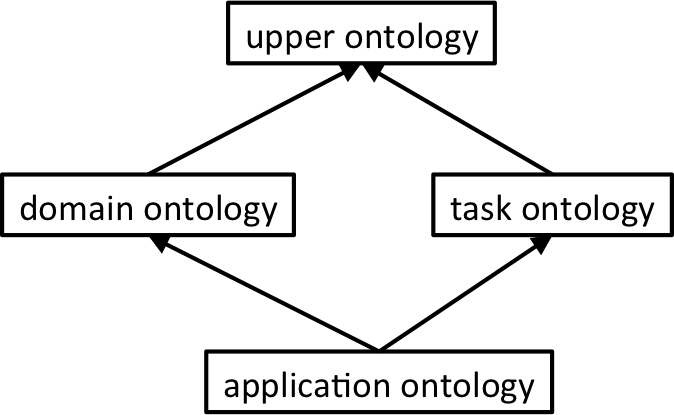
\includegraphics[width=0.45\textwidth]{images/chap-general-background/ontologies-level-dependence.png}
 \fdireta{Guarino1997a}
\end{figure}

\begin{itemize}
\item \emph{upper ontologies} describe what exist in the world, using very general concepts like space, time, matter, objects, events, actions, among others. The description of concepts in this type of ontology is independently of the problem or domain. These ontologies should always be used in conjunction with other ontologies. Examples of upper ontologies are Standard Upper Ontology (SUO) \cite{PeaseNiles2002}, Suggested Upper Merged Ontology (SUMO) \cite{PeaseNilesLi2002}, and Cyc / OpenCyc \cite{MatuszekCabralWitbrockDeOliveira2006}.

\item \emph{domain ontologies} and \emph{task ontologies} describe, respectively, the vocabulary related to a generic domain (i.e. vehicles and places) and activity (i.e. repairing and traveling). The domain ontologies define a vocabulary with common terms for reuse and sharing of information for a specific domain. In the task ontologies, the vocabulary is associated with the problem solving, independent of domain.

\item \emph{application ontologies} describe concepts depending both on the particular domain (domain ontology) and task (task ontology). These concepts often correspond to roles played by domain entities while performing a certain activity with the resolution of a problem. The concepts defined in this type of ontologies are often described by specializations of domain and task ontologies.
\end{itemize}



\subsubsection{Lightweight Ontologies and Heavyweight Ontologies}
\label{subsubsec:lightweight-ontologies}

Based on the level of formal representation, ontologies can be classified in lightweight ontologies and heavyweight ontologies. As we can see in \autoref{fig:spectrum-ontologies}, at one extreme, there are lightweight ontologies that consist of terms with little or no specification of the meaning. At the other end of the spectrum, we have heavyweight ontologies that comprise ontologies rigorously formalized by logical theories. As we move along the continuum, the amount of meaning specified and the degree of formality increases, reducing possible ambiguities \cite{UscholdGruninger2004}.

\begin{figure}[htb]
 \caption{The spectrum of lightweight and heavyweight ontologies}
 \label{fig:spectrum-ontologies}
 \centering
 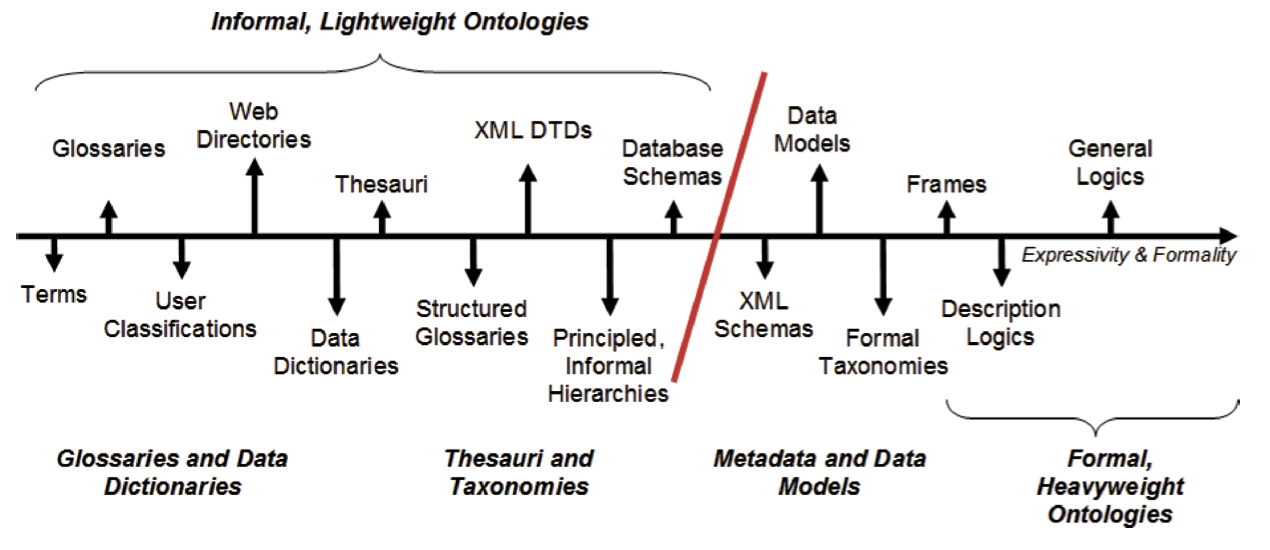
\includegraphics[width=0.9\textwidth]{images/chap-general-background/spectrum-ontologies.png}
 \fdireta{WongLiuBennamoun2012}
\end{figure}

The \emph{ligthweight ontologies} are ontologies based on topical hierarchies with lack rigorous conceptual definitions, principled conceptual organization, and label-concept distinctions. As instance of this kind of ontologies, we have terms, glossaries, thesauri, and database schemas. The main purpose of this kind of ontology is to provide a weak categorization of content to improve search engine functionality. Thus, the ligthweight ontologies are broadly used on the Web to categorize a large amount of data, such as available data on Web portals. However, these ontologies tend to be very usage-dependent and user-dependent of applications.

The \emph{heavyweight ontologies} are much more than just lightweight ontologies. They are ontologies enriched with axioms for semantic interpretation of concepts and relations. Thus, the development of heavyweight ontologies needs a rigorous definition of concepts, an organization of defined concepts based on philosophical principles, a precise and formal semantic definition of relations among concepts, and so on. Heavyweight ontologies are important to create shareable and reusable knowledge bases, because they give more value to concepts represented on them by providing greater semantic precision and ensuring the fidelity and consistency of concepts about a target world.

In this dissertation, we will develop the ontology OntoGaCLes as a heavyweight ontology, and application ontology for the domain of gamified CL scenarios.

\subsection{Ontology Representation}
\label{subsec:ontology-representation}

Nowadays, the ontologies can be represented in two ways, one representation is the formal representation that is used for computer consumption, and another representation is the graphical representation for human comprehension.

\subsubsection{Formal Representation}
\label{subsubsec:formal-representation}

To allow the formal representation for a direct computer consumption, there are many languages that have been proposed using the predicate logics, description logics or frame based languages. The most popular language and framework to describe ontologies is the Web Ontology Language (OWL) language that is based on the Resource Description Framework (RDF)/RDF-Schema.

The RDF specification was developed by the World Wide Web Consortium (W3C) for metadata description. It is formally represented in the eXtensible Markup Language (XML) employing triplets that contain a subject node, predicate, and object node ($<$subject, predicate, object$>$). Each node in the triplet can be a web resource (URI reference), a value (literal) or a document identifier (to represent a blank node). A set of triples also can become a node itself, and a property is a semantic relation between nodes (subject and object).

To represent triplets, the RDF/RDF-Schema specifications define classes, properties, and relationships that can be used to describe these triples as statements about resources. It also includes definition of tags and hierarchical structures (taxonomy) providing the basic elements for the description of ontologies. However, the RDF-Schema has some limitation, especially to support computational reasoning on data available through the internet \cite{Patel-Schneider2005}. Thus, the OWL specification provides an expressive language to develop ontologies.

OWL is a language developed and endorsed by the W3C to satisfy the formalism for the Semantic Web (SW). It allows the SW applications to understand and answer queries of agents (people or other programs) by reasoning on Web content by ontological descriptions. OWL was developed based on DAML+OIL \cite{Horrocksothers2002} with a formal specification influenced by description logics, the frames paradigms and the OWL exchange syntax (namely RDF/XML) \cite{HorrocksPatel-SchneidervanHarmelen2003}.

There are three variants of OWL referred as OWL Lite, OWL DL and OWL Full. These three variants allow to achieve a good balance between scalability and expressive power. According to the OWL specification, each variant is an extension of its simpler predecessor. Thus, OWL Lite is used manly for classification hierarchy and simple constraints; OWL DL gives maximum expressiveness retaining computational completeness and decidability; and OWL Full gives maximum expressiveness, however with no computational guarantees, the reasoning process using OWL Full may not be completed in a finite time. \autoref{fig:owl-example} shows as example part of an ontology to represent the formalization of bicycle in OWL language.


\begin{figure}[htb]
 \caption{Part of bicycle ontology in the OWL}
 \label{fig:owl-example}
 \centering
 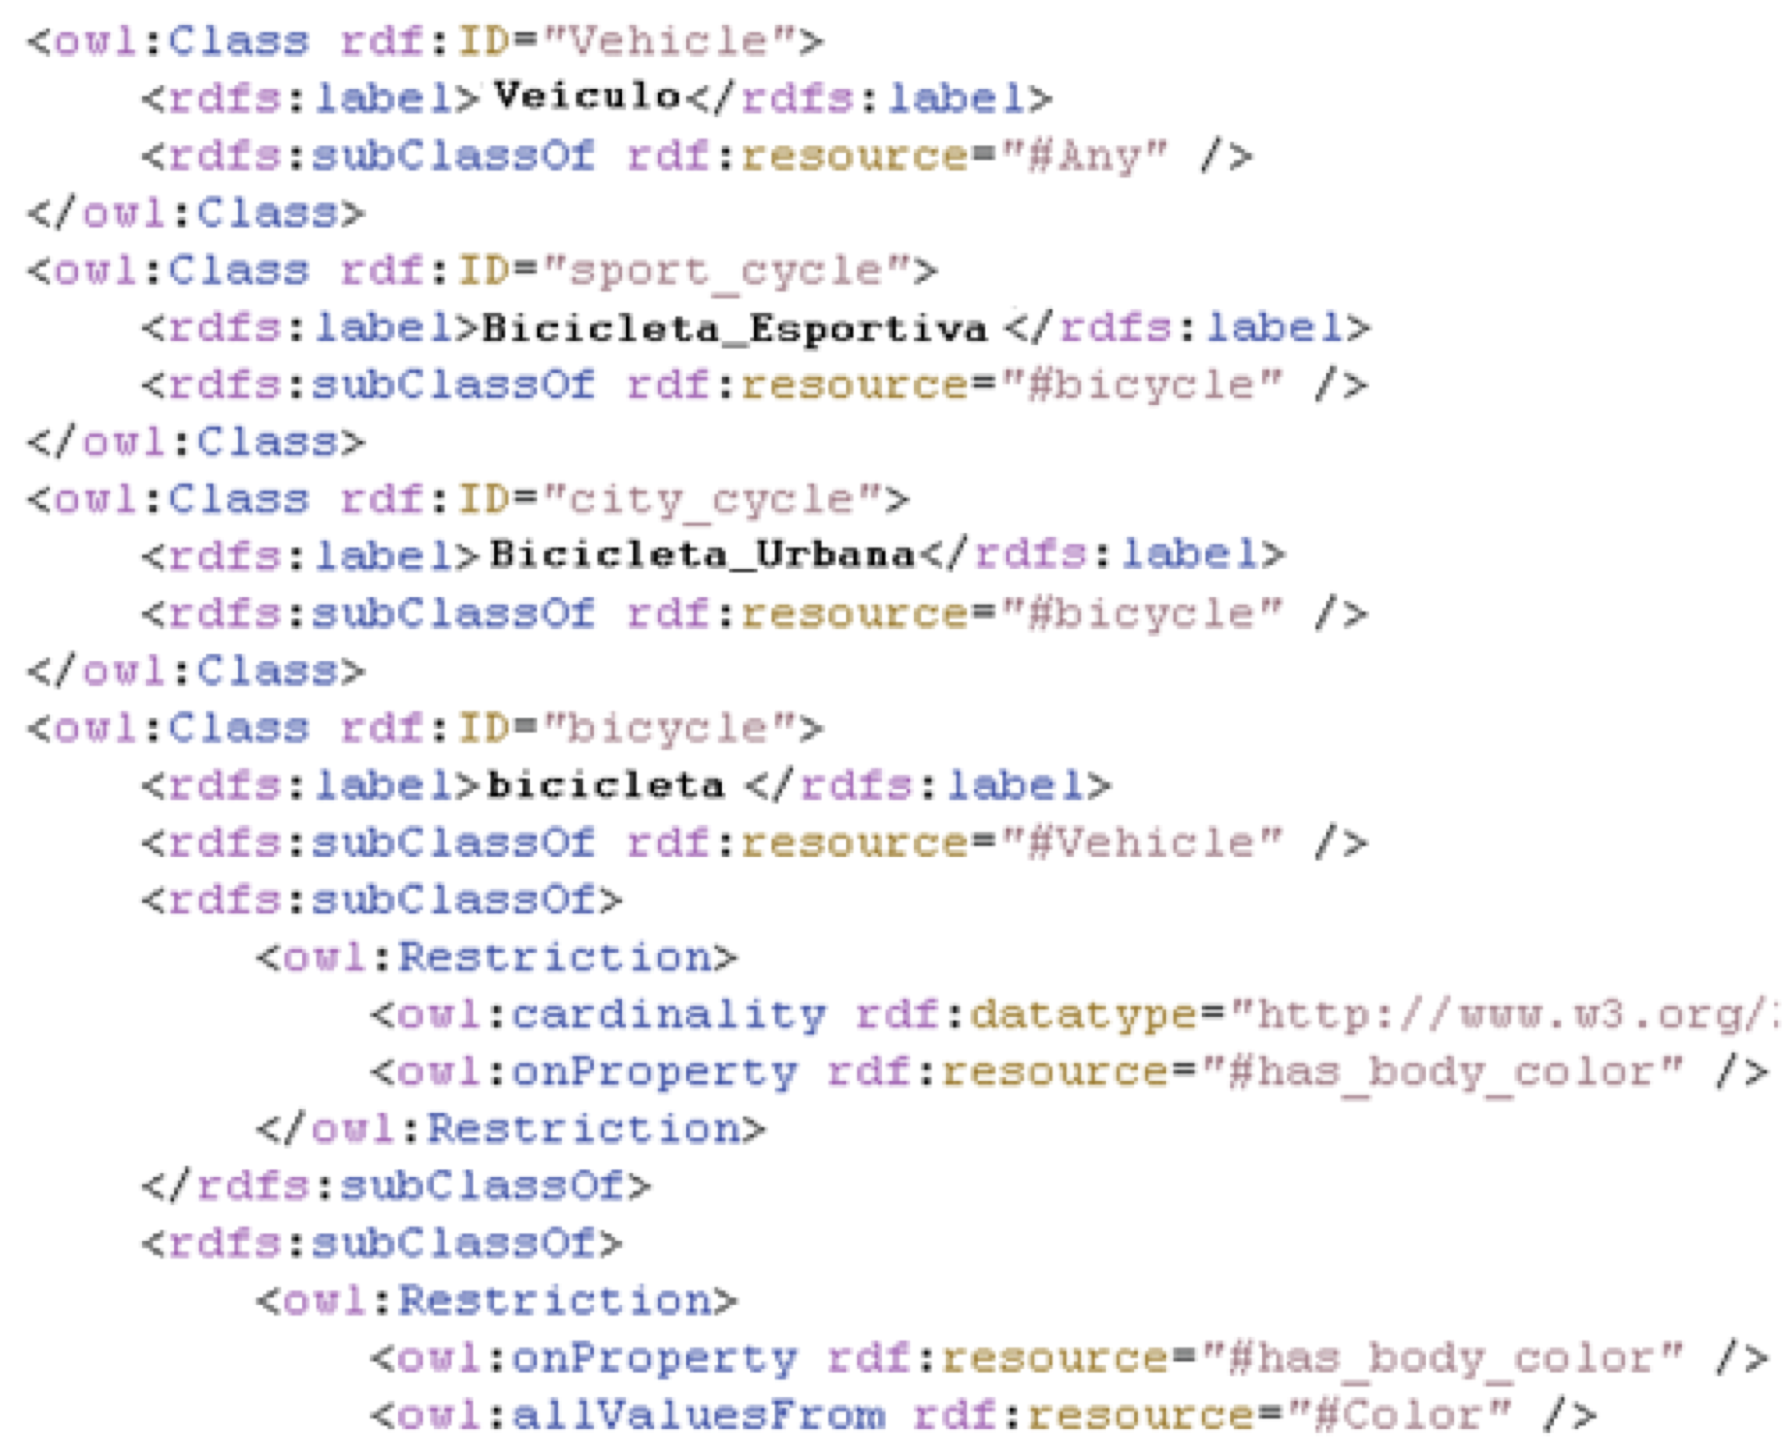
\includegraphics[width=0.8\textwidth]{images/chap-general-background/owl-example.png}
 \fdireta{Isotani2009}
\end{figure}


As the author of this dissertation used the graphical representation to describe the ontological structures, details of the RDF/RDF-Schema and OWL languages are not detailed in this section. The RDF/RDF-Schema and OWL are automatically generated by graphical ontology editors, such as Prot\'{e}g\'{e} \cite{NoySintekDeckerCrubezyFergersonMusen2001}, OntoEdit \cite{SureErdmannAngeleStaabStuderWenke2002} and Hozo \cite{KozakiKitamuraIkedaMizoguchi2002}.

\subsubsection{Graphical representation}
\label{subsubsec:graphical-representation}

As an ontology is mainly composed by concepts and their relations, the graph is a common representation of ontologies, where the nodes represent concepts and the arrows represent relations between concepts \cite{DiengHug1998}. \autoref{fig:graph-bicycle-ontology} shows the graphical representation of an ontology referred to bicycle. In this ontology, the concept of a bicycle is a specialization of vehicle represented using \emph{is-a} relation ($<$bicycle \emph{is-a} vehicle$>$). In this ontology, the class \aspas{\emph{City bicycle}} and \aspas{\emph{Sport bicycle}} are related to the class \aspas{\emph{Bicycle}} by the arrows \aspas{\emph{is-a}} to indicate that the bicycle is specialized into sport bicycle and city bicycle, and the class \aspas{\emph{Bicycle}} is associated to the class \aspas{\emph{Vehicle}} by the arrows \aspas{\emph{is-a}} to indicate that vehicle is a super-class of the class bicycle. The attributes \aspas{\emph{Color}} and \aspas{\emph{Weight}} are indicated by the arrows \aspas{\emph{attribute-of}.} Finally, the arrows \aspas{\emph{part-of}} indicate the elements that compose a bicycle, and these elements are: \emph{Wheel}, \emph{Handlebar}, \emph{Frame}, and \emph{Pedal}. The scheme of colors in this figure helps the reader identify the relationship between concepts.

\begin{figure}[htb]
 \caption{A graph representation of a bicycle ontology}
 \label{fig:graph-bicycle-ontology}
 \centering
 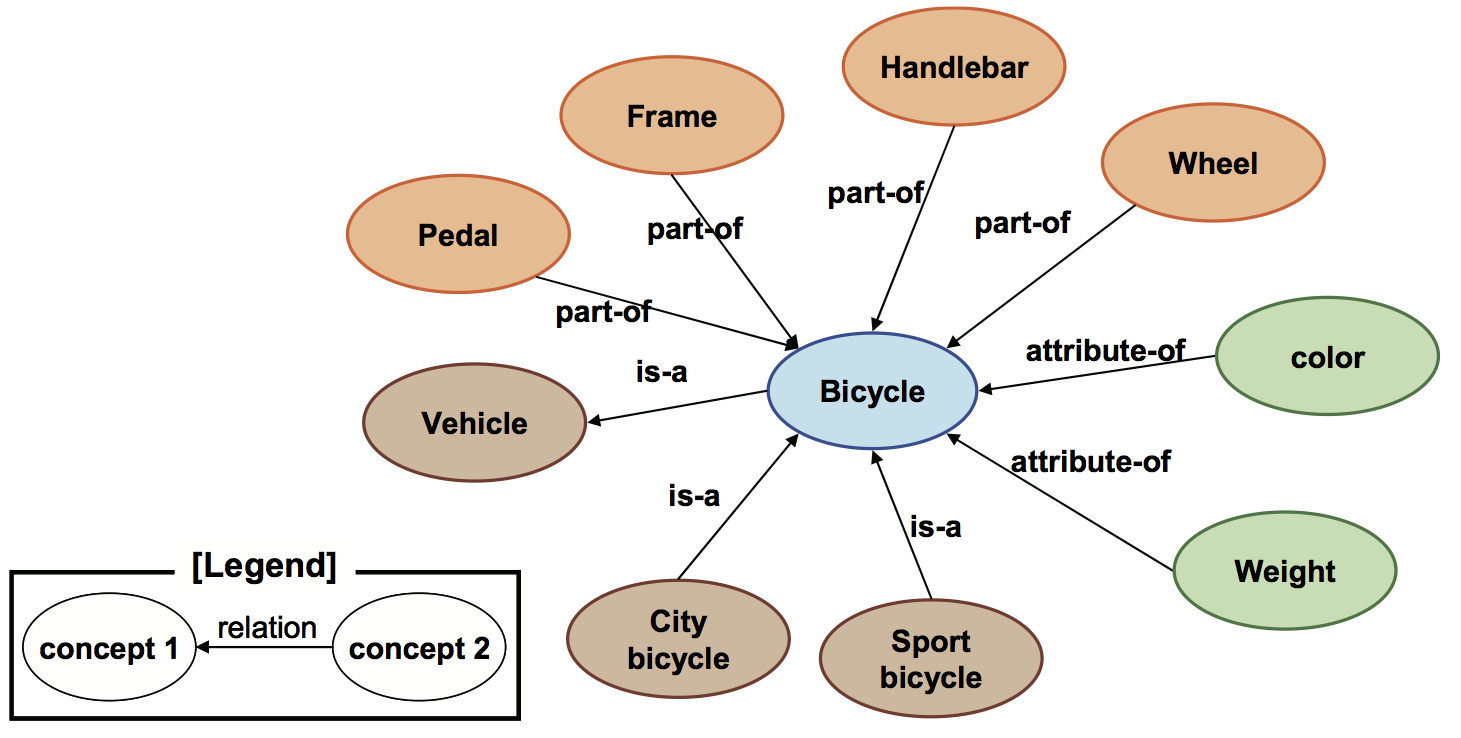
\includegraphics[width=0.8\textwidth]{images/chap-general-background/graph-bicycle-ontology.png}
 \fdireta{Isotani2009}
\end{figure}

Although the representation of ontologies using graphs is the most common, it suffers deficiencies that do not help to capture important elements in an ontology \cite{Devedzic2006}, especially when trying to represent the model of roles proposed by \citeonline{MizoguchiSunagawaKozakiKitamura2007}. 

To deal with the modeling of ontologies based on the model of role, the Hozo ontology editor \cite{KozakiKitamuraIkedaMizoguchi2002} has been proposed as an authoring environment in which the differentiating of basic concepts (e.g. human, and artifact) from role concepts (e.g. learner, and reward) is described as frames diagrams. In this graphical representation based on frames, to deal with the concept of role, the following three classes are defined:

\begin{description}
  \item[Role concept] - A concept representing a role that depends on a context (e.g. learner role that depends on the school);
  \item[Basic concept] - A concept that does not need other concepts to be defined (e.g. human); and
  \item[Role holder] - An instance of a base concept that is holding the role (e.g. learner). 
\end{description}

The basic concepts are used as class constraints, and the instances that satisfy the class constraints play the role, becoming role holders. For example as shown in the \autoref{fig:learner-role-hozo}, \aspas{In a learning environment there is a vacancy for a learner, and a person, whose name is Geiser, fills the position, becoming a learner in the particular environment.} The person who plays a role is referred as a role holder. Thus, \emph{Geiser} becomes a \emph{learner} in the \emph{learning environment} by playing the \emph{learner role}. The top of the figure shows how the concepts around a role are related to each other and in the bottom is shown the representation in Hozo.


\begin{figure}[htb]
 \caption{The learner role holder in Hozo representation}
 \label{fig:learner-role-hozo}
 \centering
 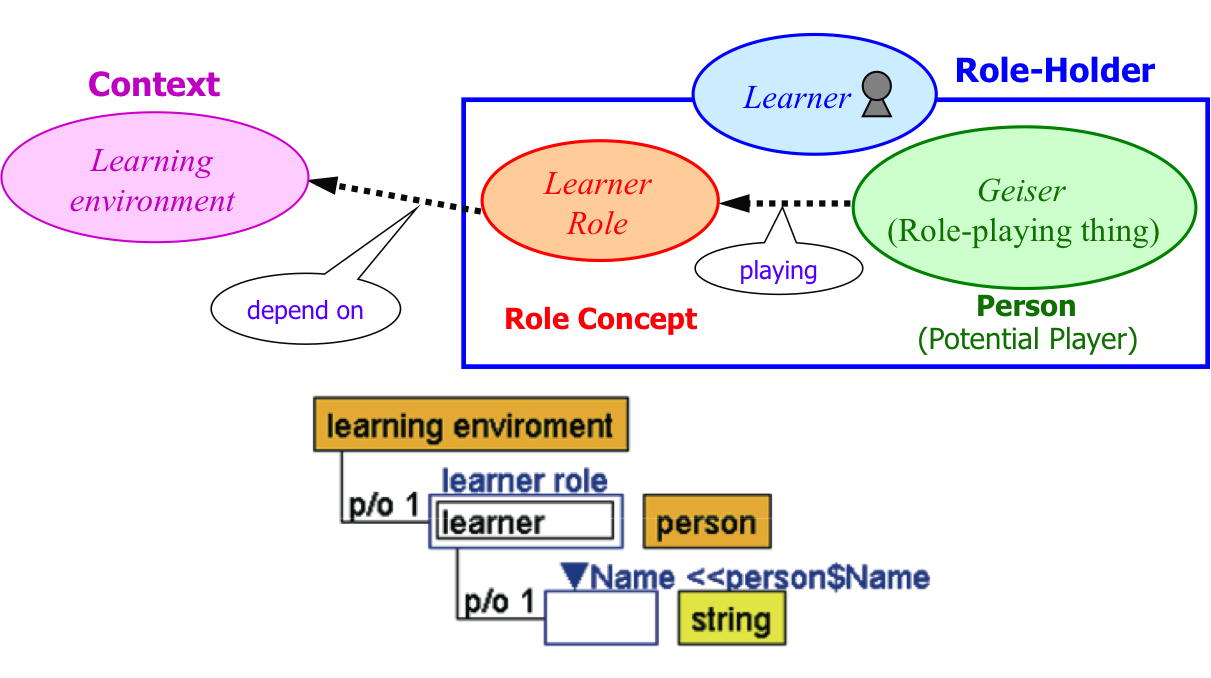
\includegraphics[width=0.8\textwidth]{images/chap-general-background/learner-role-hozo.png}
 \fautor
\end{figure}

\autoref{fig:hozo-bicycle-ontology} shows the representation of bicycle ontology using Hozo representation. In this figure, the relations part-of and attribute-of is respectively represented by labels \aspas{\emph{p/o}} and \aspas{\emph{a/o}} that appear in front of each slot. Thus, the frame, pedal, handlebar, and wheels are part of the bicycle. Observe that in the context of bicycle, a wheel (basic concept) can play the role of front wheel or rear wheel (role concepts). Thus, a particular instance of a wheel that plays one of these roles (front wheel role or rear wheel role) is referred to as role holder. In summary, a front wheel is an instance of wheel playing the front wheel role.

\begin{figure}[htb]
 \caption{Example of bicycle ontology using Hozo representation}
 \label{fig:hozo-bicycle-ontology}
 \centering
 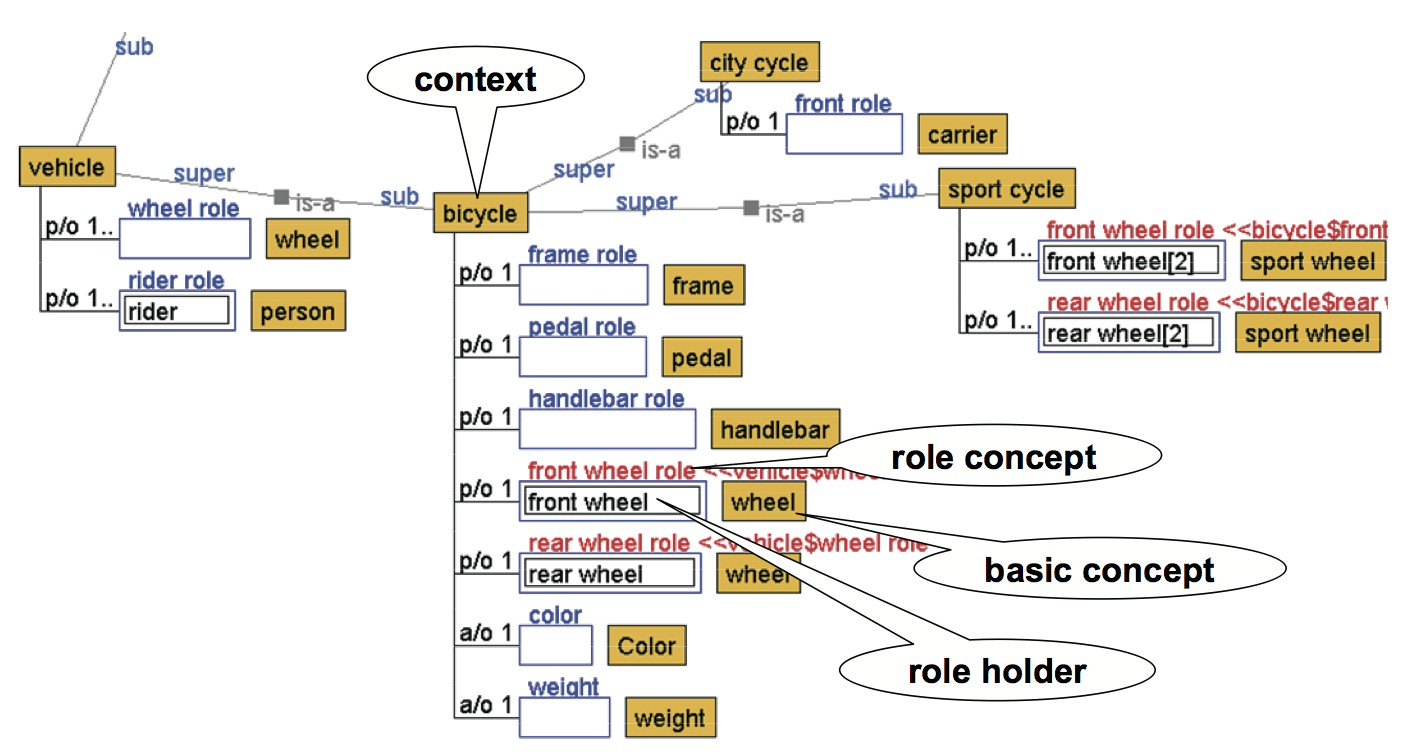
\includegraphics[width=1\textwidth]{images/chap-general-background/hozo-bicycle-ontology.png}
 \fdireta{Isotani2009}
\end{figure}

\subsection{Ontology Engineering}
\label{subsec:ontology-engineering}

Ontology engineering encompasses a set of activities conducted during the conceptualization, design, implementation and deployment of ontologies \cite{Devedzic2002,Devedzic2006}. It covers topics including philosophy, metaphysics, knowledge representation formalisms, development methodology, knowledge sharing and reuse, knowledge management, business process modeling, common sense knowledge, systematization of domain knowledge, information retrieval from the Internet, standardization, and evaluation.

Developing ontologies is a time-consuming and difficult task that requires knowledge about the target domain, theoretical background on ontology formalization, and the skills to properly define the concepts and elements as body of knowledge in ontologies. Thus, to facilitate the development of ontologies, there are several formal methodologies and methods that have been proposed. The guidelines of these methodologies and methods are categorized into three layers shown in \autoref{fig:three-layer-model} \cite{Mizoguchi2004}, in which:

\begin{enumerate}
\item \textbf{Top-layer} contains the coarsest level of guidelines that specifies the whole building process with standard software development life cycles. The guidelines described in this layer correspond to ontological methods and methodologies associated with conventional software development processes and practices.

\item \textbf{Middle-layer} describes the generic constraints and guidelines that specify a set of major steps and their order of execution. In each step of middle layer, the detailed information about the activities to be completed, and the way for each activity should be carried out. 

\item \textbf{Bottom-layer} corresponds to the most fine-grain guidelines that enable the construction of concepts hierarchy. It describes guidelines to create explicit semantic structures from identified concepts in the target world.
\end{enumerate}


\begin{figure}[htb]
 \caption{Three-layer classification model of guidelines proposed in methodologies and methods to develop ontologies}
 \label{fig:three-layer-model}
 \centering
 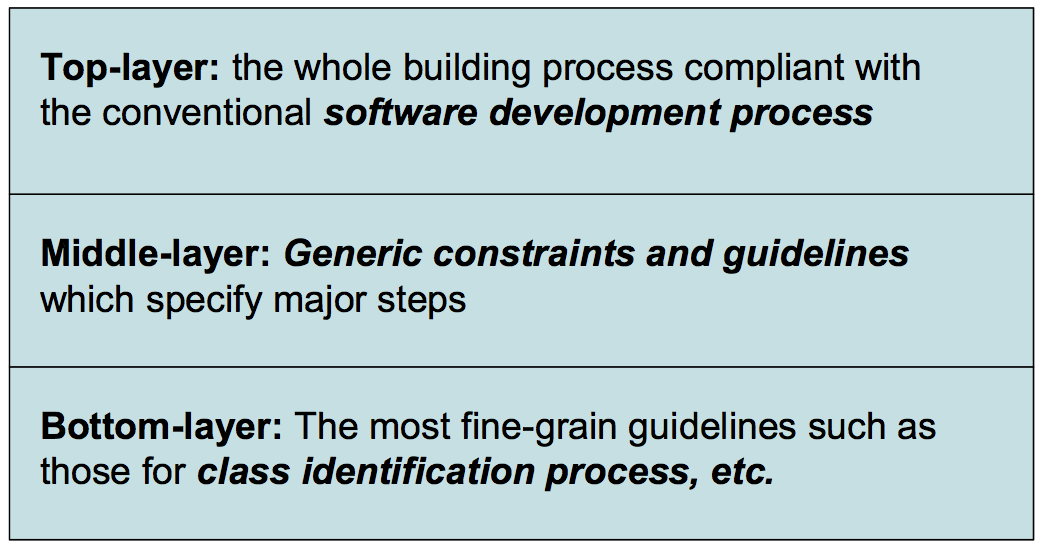
\includegraphics[width=0.7\textwidth]{images/chap-general-background/three-layer-model.png}
 \fdireta{Mizoguchi2004}
\end{figure}

Most of the currently existing methods and methodologies describe guidelines concerned mainly with the top-layer. Some examples are METHONTOLOGY \cite{Fernandez-LopezGomez-PerezJuristo1997}, On-To-Knowledge \cite{SureStaabStuder2004}, and Ushold and King's methodology \cite{UscholdKing1995}. Unfortunately, only a few of them deal with the middle and bottom layers.  The main problem of having few methodologies for the development of the middle and bottom layers is that the chances of creating a good ontology at the end of some process decreases.

In this sense, \citeonline{Mizoguchi2004} proposed a set of guidelines to support the development of ontologies at the middle and bottom layers based the Activity-First Method \cite{Mizoguchi1995}, and in this dissertation, the author of this dissertation utilized these guidelines to create the ontology OntoGaCLeS. Therefore, the rest of this section presents an overview of guidelines \cite{Mizoguchi2003,Mizoguchi2004a,Mizoguchi2004} that were summarized by \citeonline{Isotani2009} as described as follows:

\subsubsection*{Middle Layer Guidelines}
\label{subsubsec:middle-layer}

\begin{enumerate}
\item Identify concepts rather than terms. As ontology is totally independent of terminological problems, one cannot stress the importance of this distinction too much. Since people will be easily trapped by the endless terminological discussion departing from the underlying conceptual structure of the target domain.

\item Use mixed and flexible strategies of top-down, bottom-up and middle-out. Never stick to only one of the strategies. 

\item Whenever possible, identify and use top-level ontology in the early phase of the development process to govern the rest of the steps. 

\item When you deal with a concept, identify its main components, using \aspas{\emph{part-of}} relation as well as its main attributes. You can thus find and extend candidates of concepts to be included in the ontology. 

\item Definition of axioms should be done after finishing is-a hierarchy building and informal term definition. 

\item Note that you cannot define any concept completely in theory. Therefore, do not stick to the definition of each term too much. At the best, you only can give necessary conditions of them. Term definition in the early phase can be rough. Detailed definition of a term should be done after you grasp the whole structure of the ontology, that is, after building is-a hierarchy. 

\item Never try to seriously define a term one by one. Definition of a concept needs sufficient contextual information, which is usually not available in the early phase. Terms are related to each other and could have several meanings, which should be clarified by the context given. 

\item Arrange and resolve the terminological issues (how to name a concept) at the last step. 

\item When you find the necessity to define more than one meaning for one term, then you are facing the terminological problem. Each term should correspond to exactly one concept in ontology, since you are not building a dictionary, but a well-organized conceptual structure. Each term is only a label of the concept. You of course can build a dictionary after building ontology.

\item Put a higher priority on is-a hierarchy construction than term definition. Carefully designed is-a hierarchy gives you a correct context to define a term.

\item When you get stuck with a term definition, follow either one of the following : 
\begin{itemize}
\item Multiple meanings? Then concentrate on meaning one by one. 
\item Multiple Viewpoints? Make the viewpoint explicit and then try it again 
\item Check if you are discussing terminology.
\item Use is-a hierarchy to give enough context. 
\end{itemize}
\end{enumerate}

\subsubsection*{Bottom Layer Guidelines}
\label{subsubsec:bottom-layer}

\begin{enumerate}
\item \emph{Identify essential properties} for each concept considered essential in the scope of a given problem. These essential properties facilitate to create more stable concepts and hierarchies during the ontology development process.

\item \emph{Make correct use of the role-concept} that can be defined as the association of a concept to a particular role within a given context. When developing an ontology, one should carefully distinguish the difference between role-concept, role-holder, and basic concepts. Such differentiation helps to treat multiple meanings as introduced previously in the guidelines for the Middle layer.

\item \emph{Be careful when using is-a relation} in ontologies is different from the one utilized by object- oriented programming. The is-a relation applies only for classes. Furthermore, for given classes A and B the relation $<$class A is-a class B$>$ is true if and only if the instance set of A is a subset of the instance set of B. Therefore building a relation such as $<$teacher is-a human$>$ is ontologically incorrect, since \emph{teacher} is not an ontologically-valid class because there is no person (no instance of class person) whose intrinsic property is being a teacher. Thus, in ontology, it is inappropriate to model $<$Mizoguchi instance-of Teacher$>$ and $<$Teacher is-a Human$>$.% (What happens if Mizoguchi quits his job?).

\item \emph{Be careful when using part-of relation} such as functional, qualification, spatial and etc. Thus, it needs to be used carefully, especially avoid part-of relation to create class hierarchies such as $<$man part-of human$>$. Such an expression is valid only when you want to deal with man as a subspecies of human.

\item \emph{Pay attention to the difference between is-a and part-of relations}. Usually, the meaning of is-a and part-of relations is easy to distinguish. The former indicates generic vs. specific relations between classes. The latter is often utilized to specify the composition of a thing (although, part-of can be used in other situations). However, sometimes when developing an ontology, one can encounter difficulties to distinguish their difference. For example, which of the following relation is correct: $<$Dog part-of mammal living in Japan$>$ or $<$Dog is-a mammal living in Japan$>$? People agree that $<$Dog is-a mammal$>$ is correct. However, by adding the \emph{living in Japan} phrase to mammal the distinction is not quite that easy because \emph{mammal living in Japan} seems to represent species, and therefore, $<$\emph{dog-species} part-of  \emph{mammal-species} living in Japan$>$ could be considered. Thus, the distinction between is-a and part-of relation is not always easy.

\item \emph{Avoid the use of multiple inheritances} Creating multiple inheritances is the source of many problems to keep the consistency of the representation. In particular, propagating the essential properties is a problem since each concept should be recognized and represented by their own essential properties.

\item \emph{Some boundary between similar concepts can be vague} When developing an ontology some boundaries between similar concepts do not need to be strongly conceptualized. An example is the distinction between the concepts black and white. Since the distinction between them is based on the ambiguous color gray, we cannot give a clear and unique boundary between black and white (although we recognize their existence).

\item \emph{Create terms if there is no label to represent a concept}. If you cannot find an appropriate term to represent a concept, then you can temporarily label them with some sentences or marks (e.g., concept 1 and concept 2) until you can come up with a good label. When the body of the ontology is good enough to represent the target domain, you can revise the labels of each concept.
\end{enumerate}

